\documentclass[11pt,a4paper]{article}

\usepackage[margin=2.5cm]{geometry}
\usepackage[T1]{fontenc}
\usepackage[utf8]{inputenc}
\usepackage{lmodern}
\usepackage{microtype}
\usepackage{booktabs}
\usepackage{array}
\usepackage{graphicx}
\usepackage{amsmath}
\usepackage{amssymb}
\usepackage{xcolor}
\usepackage[hidelinks]{hyperref}
\setlength{\emergencystretch}{3em}

% ---------- Macros ----------
% Placeholder for the result of the reproduction check (still running when this draft was written).
\newcommand{\REPRO}{\textcolor{red}{[reproduction result pending]}}
% Placeholder for facts that the release step must add.
% Model names and metric names are Technical Names. \M escapes nothing: write + and - as they are.
\newcommand{\M}[1]{\texttt{#1}}
\newcommand{\ura}{\texttt{unseen\_\allowbreak rule\_\allowbreak accuracy}}
\newcommand{\cpa}{\texttt{counterfactual\_\allowbreak paired\_\allowbreak accuracy}}
\newcommand{\pcons}{\texttt{paraphrase\_\allowbreak consistency}}
\newcommand{\ooi}{\texttt{option\_\allowbreak order\_\allowbreak invariance}}
% Table helpers: mean +- std, a difference with its CI, and the marks of the CI against A.
\newcommand{\ms}[2]{$#1 \pm #2$}
\newcommand{\ci}[3]{$#1$ [$#2$, $#3$]}
\newcommand{\up}{\textsuperscript{$+$}}
\newcommand{\dn}{\textsuperscript{$-$}}
\newcolumntype{R}[1]{>{\raggedleft\arraybackslash}p{#1}}
\newcommand{\hash}[1]{{\ttfamily\scriptsize #1}}

\title{Does Rule Conditioning Help a 17M Encoder Decide on Unseen Rules?\\
A Negative Result for the CRUX Architectures}
\author{Antony Ranjith F.}
\date{Draft of 22 October 2026}

\begin{document}
\maketitle

% =====================================================================
\begin{abstract}
\noindent
Compact models can make fast rule-based decisions on a device, but they must work with rules that they did not see in training.
The CRUX project tests this hypothesis: explicit rule-conditioned computation, together with counterfactual learning, helps a small encoder generalize to unseen rules better than a plain encoder classifier.
We build four architectures on the Ettin-17M encoder.
Architecture A is the plain baseline.
Architecture B adds an instruction-conditioned low-rank hypernetwork.
Architecture C adds counterfactual training and a consistency loss.
Architecture D adds cacheable state and instruction representations and a permutation-equivariant set-attention block.
We add seven controls and ablations.
We compare all models under one protocol with pre-registered seeds, metrics, and statistics: 3 seeds, the same training budget (12000 steps, one hyperparameter trial, set after a 6000-step pilot), and a 95\% paired bootstrap CI.
We train on a new synthetic generator whose labels a symbolic rule engine verifies, and we test on held-out templates, rule compositions, and vocabulary.

The result is negative.
No architecture is reliably better than A.
On the test split with unseen rules, B equals A on \ura{} (difference $-0.004$, 95\% CI $[-0.010, +0.001]$) and is $0.009$ lower on \cpa{} (CI $[-0.016, -0.001]$).
All other models are reliably worse than A.
D is $0.198$ lower than A.
At this budget, our form of counterfactual batches decreases the accuracy of A and of B.
The split encoding that makes D cacheable decreases the validation accuracy by $0.058$ to $0.113$, and the cache does not reduce the latency at batch size 1 below the latency of A.
On the ProofWriter test sets and on three external benchmarks, the models are at, near, or below the majority baseline, so we find no evidence of transfer.
We did not evaluate the external baselines Ettin-32M and DeBERTa-v3-xsmall, we did not evaluate Jev, and we did not make any on-device or INT8 measurement.
The result holds for 3 seeds, one trial, and 12000 steps.
We release the code, the configurations, and the split hashes.
\end{abstract}

% =====================================================================
\section{Introduction}

A System 1 decision model gives a fast answer to a question about facts and rules.
The CRUX project builds a compact System 1 decision model that is inspired by Jev of TypeSafe AI.
Jev has no public weights, and it has only self-reported results.
The CRUX project asks if a small open model, with about 17M to 30M parameters, can do this task and run on a mobile device.
The central difficulty is generalization: a deployed rule set differs from the training rule sets.

The research hypothesis of the project is as follows.
\emph{Explicit rule-conditioned computation, combined with counterfactual learning, can enable small neural networks to generalize to unfamiliar decision tasks more effectively than conventional transformer-based classifiers.}
The project fixes a success criterion before training: a statistically reliable improvement over the baseline A in held-out rule generalization and in counterfactual decision accuracy.
An improvement is reliable only if the 95\% paired bootstrap CI of the difference to A excludes 0.

We test the hypothesis with four architectures (A, B, C, D) and with controls that separate the effect of each part.
The controls matter because an improvement can come from extra parameters, from the training data, or from the loss, and not from the architecture.
The project pre-registered the seeds, the metrics, and the statistics before the first training run.
It set the training budget after a pilot with 6000 steps (Section~\ref{sec:deviations}).

\paragraph{Result.}
The hypothesis is not supported at this budget.
No architecture is reliably better than A on the primary metrics.
B equals A on \ura{} (the CI includes 0) and is $0.009$ lower on \cpa{} (the CI is below 0).
C, D, and the controls that use counterfactual batches are worse than A.
We report this result in full, with all controls, all comparisons whose CI includes 0, and all limitations.

\paragraph{Contributions.}
\begin{enumerate}
  \item A deterministic generator of decision tasks. Two independent implementations (a generator and a symbolic rule engine) agree on every label. The generator makes matched counterfactual pairs and logically equivalent paraphrases, and it holds out templates, rule compositions, and vocabulary for validation and test.
  \item A comparison of 4 architectures and 7 controls and ablations (11 models, 33 runs) with an equal training budget, under pre-registered seeds, metrics, and statistics.
  \item A negative result with the controls that explain it: the extra parameters, the counterfactual data, the consistency loss, and the two parts of D are each measured alone.
  \item The code, the configurations, and the split hashes for a reproduction.
\end{enumerate}

\paragraph{Novelty.}
We claim no novelty for any single part.
Text-conditioned hypernetworks, counterfactual data, consistency losses, split encoding with a cache, and set modules for candidates all exist (Section~\ref{sec:related}).
Only the combination of these parts at 17M to 30M parameters for compact rule decisions can be new.
We found no earlier work that joins all of them at this size in a limited search, and this paper does not prove that no such work exists.
Our results do not support a claim that the combination works.

% =====================================================================
\section{Related Work}\label{sec:related}

\paragraph{Instruction-conditioned hypernetworks.}
A hypernetwork generates the weights of another network \cite{ha2016}.
Several works condition such a network on text.
Ye and Ren generate adapters from a task description \cite{ye2021}.
Karimi Mahabadi et al.\ use a shared hypernetwork to generate adapter weights for many tasks \cite{mahabadi2021}.
HyperTuning reads few-shot examples with a hypermodel and outputs a soft prefix or LoRA weights for a frozen T5 model \cite{phang2023}.
HINT encodes the instruction once and converts it into parameter-efficient modules, so the instruction does not enter the model input again for each example \cite{ivison2023}.
Text-to-LoRA generates a LoRA adapter from a task description in one forward pass \cite{charakorn2025}.
Volk et al.\ generate the weights of a classifier from an example, to adapt to unseen domains \cite{volk2023}.
These works use T5-scale or larger models and task descriptions or few-shot examples.
In a limited search, we found no work that conditions a low-rank head on formal rule text for an encoder with 17M to 30M parameters.
LoRA is the low-rank form that architecture B uses \cite{hu2021}.

\paragraph{Counterfactual data and consistency training.}
Kaushik et al.\ ask humans to edit an example so that its label flips, and they train on both examples \cite{kaushik2020}.
Gardner et al.\ define contrast sets, small label-changing edits that test the local decision boundary \cite{gardner2020}.
Li et al.\ and Asai and Hajishirzi add logic-based consistency losses and logic-guided augmentation \cite{li2019,asai2020}.
Elazar et al.\ measure and improve the paraphrase consistency of language models \cite{elazar2021}.
Nafar et al.\ add logical-constraint losses on a probabilistic RuleTaker variant \cite{nafar2024}.
Counterfactual pairs and consistency losses are established.
Our generator differs in one detail: a symbolic rule engine verifies the label of each pair by program.

\paragraph{Rule-reasoning data sets.}
RuleTaker shows that transformers can answer questions over facts and natural-language rules \cite{clark2020}.
ProofWriter uses the same data format and adds proofs \cite{tafjord2021}.
BoardgameQA adds contradictory information, rule priorities, and missing information \cite{kazemi2023}.
DynaGuard and its test set DynaBench cover user-defined policies for guardrail decisions \cite{hoover2025}.
The DynaGuard models have 1.7B to 8B parameters.
Super-NaturalInstructions gives held-out instruction-following tasks \cite{wang2022}.

\paragraph{Cacheable and permutation-equivariant scoring.}
Bi-encoders and cross-encoders trade accuracy for speed.
Poly-encoders sit between them \cite{humeau2020}.
ColBERT encodes query and document separately and keeps token-level vectors for a late interaction step \cite{khattab2020}.
DeFormer removes the cross-attention between question and context in the lower layers, and it caches the context at some loss of accuracy \cite{cao2020}.
This is the trade-off that our \M{C+cache} ablation measures.
Deep Sets and the Set Transformer give the theory and the attention modules for set inputs \cite{zaheer2017,lee2019}.
A multiple-choice head that scores each candidate with shared weights is already permutation-equivariant \cite{zellers2018}.
Decoder language models are sensitive to the order of options \cite{zheng2024}.
Only an extra step across candidates, for example a Set Transformer block, adds something to the standard head.

\paragraph{Small encoders.}
Ettin is an open suite of paired encoders and decoders from 17M to 1B parameters \cite{weller2026}.
Ettin-17M is the base of all our models.
ModernBERT is the encoder recipe on which Ettin builds \cite{warner2025}.
DeBERTa-v3 is the second small encoder that the protocol names as an external baseline \cite{he2023}.

% =====================================================================
\section{Task and Unified Decision Schema}\label{sec:task}

Each data set becomes a list of decision records with the fields \texttt{state}, \texttt{instruction}, \texttt{options}, and \texttt{target}.
The \texttt{state} holds the facts and the evidence.
The \texttt{instruction} holds the rules and the question.
The two fields stay separate, because architecture D encodes and caches them independently.
The \texttt{options} field is a list of two or more candidate answers.
The \texttt{target} field is the index of the correct option.

The schema has three task types.
A binary task has a fixed label set for the whole source.
All sources use one canonical order: the positive label, the negative label, then ``Unknown'' (for example True, False, Unknown).
A multi-choice task has options that change from record to record.
A scoring task gives a graded value to each option.
No current data set needs the scoring type, so we do not use it in the experiments.
All task types share the candidate form: a list of options and a target that points into it.

Every model scores each option as one sequence \texttt{[CLS] state [SEP] instruction [SEP] option [SEP]} with one scalar.
The softmax over the real options of a record gives the probabilities, and the prediction is the argmax.
A binary record with the three labels True, False, and Unknown has three option sequences.
Architecture D uses a different input form (Section~\ref{sec:models}).
The code truncates the rules and keeps the question whole.
We checked truncation in three ways: in separate mode, the full train and validation splits have 0 truncated records; in joint mode, a sample of 2{,}000 synthetic records has 0 truncated records; and the Step 8 evaluation, with larger limits, truncates 0 records in all sets.

% =====================================================================
\section{Data}\label{sec:data}

\subsection{Counterfactual generator}

The generator makes the training, validation, and test records in the synthetic split.
The data have an \emph{open-world} semantics with classical negation: a value is true, false, or unknown, and a missing fact means unknown.
A \emph{theory} has entities, boolean and integer attributes, facts, rules, exceptions, and priorities.
Rules apply to each entity separately.
An exception blocks one rule.
A priority decides between two firing rules with opposite conclusions.
The generator rejects a theory with an unresolved conflict.

A theory has five rule-type features: \texttt{conj} (a rule with two or more conditions), \texttt{neg} (a negated condition), \texttt{thr} (a threshold on an integer attribute), \texttt{exc} (an exception), and \texttt{pri} (a priority).
The set of present features gives one of 32 compositions (\texttt{c00} to \texttt{c31}).
The depth of a query is the length of the shortest derivation of its answer (for an Unknown label, the height of the queried attribute).
The generator makes binary records (labels True, False, Unknown) and multi-choice records with 2 to 8 options.

A \emph{unit} is one original theory, one counterfactual edit of it, one query, and one to three templates.
An edit changes exactly one part of the theory.
The eight edit types are \texttt{fact\_flip}, \texttt{fact\_remove}, \texttt{fact\_number}, \texttt{threshold\_shift}, \texttt{exception\_remove}, \texttt{priority\_swap}, \texttt{rule\_remove}, and \texttt{condition\_negate}.
The first three change the state.
The other five change the rules.
The rule engine computes the labels of both members of a pair, so a pair is a \emph{flip} (the label changes) or a \emph{stay} (the label does not change).
A paraphrase renders the same theory and query with another template of the same template group, so a paraphrase is logically equivalent by construction.

The output has 100{,}000 records: 69{,}930 binary and 30{,}070 multi-choice.
The share of flips among the pairs is $0.600$.
The generator uses 15 template families in 5 groups of 3, and 12 vocabulary pools (one pool is one decision domain).
The rule engine (\texttt{crux/gen/engine.py}) and the generator are independent implementations.
They agree on all 100{,}000 records and on 70{,}000 random fuzz theories.
An audit with 41 checks of shortcuts and invariants passes on the final data.
Two runs of the generator give the same SHA-256 hash.
The vocabulary pools and the templates avoid the tokens and phrases of BoardgameQA, RuleTaker, and ProofWriter.

\subsection{Splits}

A validation or test record may use a template, a composition, a vocabulary pool, or a paraphrase only if the training split does not contain it.
The generator draws all identifiers of a unit from one block (train, validation, or test).
Table~\ref{tab:splits} lists the splits.
Validation holds out the compositions \texttt{c05}, \texttt{c08}, \texttt{c11}, and \texttt{c23}.
The test block holds out \texttt{c18}, \texttt{c28}, and \texttt{c31}.
The 7 held-out compositions are stratified by the number of rule-type features.
Reasoning depths 4 and 5 occur only in validation and test.
The training split has depths 0 to 3.
The split \texttt{dev\_id} is an in-distribution development set made from 5\% of the training-block units.
It is not used for model selection.
We use it to compare the accuracy on seen rules with the accuracy on unseen rules.

The test split also holds three held-out ProofWriter sets in the open-world form with three classes: \texttt{depth5} (ProofWriter depth 5), \texttt{birds\_electricity} (the Birds-Electricity domain), and \texttt{pararules} (ParaRules, human paraphrases).
We use only these held-out sets from ProofWriter, and not RuleTaker or ProofWriter training data, so none of the 11 models trains on natural-language rule text in this project (the Ettin pretraining data can contain such text; Section~\ref{sec:data}).
The test split has no closed-world RuleTaker set.
The open-world ProofWriter sets stand in for it.
They are comparable only with published open-world results \cite{tafjord2021}, and not with the closed-world RuleTaker results \cite{clark2020}.

\begin{table}[t]
\centering
\caption{Frozen splits. The column ``Records'' is a count. The SHA-256 hashes are in Appendix~\ref{app:hash}.}\label{tab:splits}
\small
\begin{tabular}{lp{8.4cm}r}
\toprule
Split & Content & Records \\
\midrule
train & synthetic train block (25 compositions, depths 0--3) & 75{,}646 \\
dev\_id & synthetic, same templates and compositions as train & 4{,}162 \\
validation & synthetic, unseen templates, vocabulary, compositions & 10{,}106 \\
test & synthetic test block & 10{,}086 \\
 & ProofWriter \texttt{depth5} (open world) & 18{,}857 \\
 & ProofWriter \texttt{birds\_electricity} & 5{,}270 \\
 & ProofWriter \texttt{pararules} & 8{,}008 \\
 & \emph{test total} & 42{,}221 \\
\midrule
BoardgameQA & official test file of each of 15 subsets (evaluation only) & 15{,}000 \\
DynaBench & test set (evaluation only) & 543 \\
Super-NaturalInstructions & 41 held-out classification tasks, 100 instances each (evaluation only) & 4{,}100 \\
\bottomrule
\end{tabular}
\end{table}

\subsection{External benchmarks}

We use three benchmarks for evaluation only.
No model trains on them.
\begin{itemize}
  \item \textbf{BoardgameQA} \cite{kazemi2023}: facts, rules, exceptions, and rule priorities, with labels proved, disproved, and unknown. We use the official test file of each of the 15 subsets.
  \item \textbf{DynaBench} \cite{hoover2025}: a user-defined policy and a dialogue, with labels compliant and not compliant. The test set has 543 examples, so the CIs are wide.
  \item \textbf{Super-NaturalInstructions} \cite{wang2022}: the official held-out tasks. We keep the 47 classification tasks that have a fixed label set of 2 to 8 labels. We exclude 6 of them because their instance license is ``Unknown''. 41 tasks remain, and we use the first 100 instances of each task in file order, as in the official loader.
\end{itemize}
We exclude ShARC, because it has no known license and published work reports spurious label patterns.
Section~\ref{sec:license} gives the license of each source.

\subsection{Leakage check and contamination}

\paragraph{Leakage inside the project data.}
No identifier (template, template group, composition, vocabulary, paraphrase group, unit, theory hash) is shared between the training, validation, and test splits.
There is no exact duplicate.
The word 8-gram overlap between the evaluation sets and the training split has a maximum of $0.0000$ in all six pairs that we checked (validation, test, and the three benchmarks against train, and test against validation).
The limit is $0.10$.
The check is not vacuous: \texttt{dev\_id} against train gives a mean share of $0.596$.

\paragraph{Contamination of the pretraining data.}
The documentation of Ettin does not name RuleTaker or ProofWriter.
The documentation does not prove that the corpus is clean.
We measured the overlap directly.
We scanned the test split against all 66 files of the Dolma v1.7 \texttt{tulu\_flan} data (29.1 GB, 11.0 billion words) \cite{soldaini2024}.
The RuleTaker examples of the Super-NaturalInstructions tasks 966 and 967 occur verbatim in this corpus (591 of 596 examples flagged), so Ettin probably saw RuleTaker text (the link between the Ettin \texttt{tulu\_flan} folder and this corpus is inferred from the Dolma URL list and the token counts).
1{,}173 ProofWriter \texttt{depth5} records from 67 theories share more than $0.10$ of their 8-grams (maximum $0.2013$).
They share the RuleTaker sentence frames and names, not whole theories.
Following the pre-registered rule, we removed these records before the freeze.
\texttt{depth5} has 18{,}857 records after the removal (20{,}030 before).
Of the remaining records, 16{,}117 share at least one 8-gram with the corpus, and the maximum share is $0.10$.
The synthetic test block and Birds-Electricity share no 8-gram with the corpus.
ParaRules has a maximum share of $0.0106$.
We did not scan Super-NaturalInstructions.
The Flan catalog lists 115 of its 119 held-out tasks, so we treat it as possibly seen in pretraining.
All 11 models start from the same Ettin-17M weights, so a contamination affects them in the same way.

% =====================================================================
\section{Architectures and Controls}\label{sec:models}

All models start from the Ettin-17M encoder (7 layers, hidden size 256, 4 attention heads, global attention in layers 0, 3, and 6) \cite{weller2026}.
All parameters train.
For every model, the number of total and trainable parameters is equal.
Table~\ref{tab:models} lists the models.

\paragraph{A (baseline).}
The encoder reads each option sequence.
Mean pooling over the tokens gives one vector.
The decision head is a dense layer, GELU, LayerNorm, and a linear layer to one scalar.
A has 16{,}863{,}745 parameters.

\paragraph{B (rule compiler).}
B adds a hypernetwork.
The instruction embedding $z$ is the mean final hidden state over the instruction tokens, averaged over the options of a record.
The hypernetwork is LayerNorm, a linear layer to 64 units, GELU, and a linear layer to the factors.
It generates rank-8 factors $(U, V)$ for the dense layer of the head: $Wx + (xU)V$.
The $V$ factors start at zero, so B starts equal to A.
B adds 283{,}200 parameters.

\paragraph{B-abl.}
B-abl also generates rank-8 adapters for the attention projections (\texttt{Wqkv} and \texttt{Wo}) of the top 2 of 7 encoder layers.
A soft bound $\ell \tanh(v/\ell)$ limits the generated encoder factors.
Without it, all 3 seeds of the first B-abl run stopped with a non-finite fp16 loss.
B-abl adds 1{,}880{,}640 parameters.

\paragraph{A-param (control).}
A-param is A with a static LoRA \cite{hu2021} that has the same number of trainable parameters as the hypernetwork of B (282{,}880 more than A).
It has no instruction conditioning.
This control shows if the conditioning helps, or only the extra parameters help.
The LoRA sits on the head and on encoder linear layers, from the top layer down.
The latency of A-param includes the LoRA, which we did not merge into the weights.

\paragraph{Counterfactual batches (CF).}
The frozen training split already holds both members of every pair and 1 to 3 paraphrases of each member.
A and B train on all of these records in a random order.
The protocol requires the same data for every model, so \emph{CF is a different order of the same records}.
A batch of 32 records holds whole units: the original and the edited record of each pair are always in the same batch, and the paraphrases of a unit are in the same batch (a batch cut separates about 7.4\% of the paraphrase groups).
A batch then holds about 11 units, against 32 almost independent records for A and B.
The number of records per epoch and the number of batches per epoch (2{,}364) do not change.
This is one form of counterfactual training.
Our conclusions about CF apply to this form only.

\paragraph{C.}
C is B with CF batches, the cross-entropy loss, and a consistency loss.
The consistency loss is the mean Jensen-Shannon divergence of each paraphrase group in the batch to the mean distribution of the group, with weight 1.0.
We fixed the weight and did not search it, because the budget has one trial.

\paragraph{A+CF and B+CF (controls).}
A+CF is A with CF batches.
B+CF is B with CF batches and without the consistency loss.
A+CF separates the effect of the data order from the effect of the architecture.
B+CF separates the effect of the data order from the effect of the consistency loss.

\paragraph{D (CRUX).}
D is C with two additional parts.
\emph{Split encoding} ($J = 4$): the bottom 3 of the 7 encoder layers encode the state, the instruction, and each option as separate sequences, each as \texttt{[CLS] text [SEP]} with positions from 0.
The states of these layers do not depend on the question options or on each other, so they are the cache.
The top 4 layers (layers 3 to 6, with the two global layers 3 and 6) read \texttt{[state ; instruction ; option]} for each option.
The split encoding adds no parameters.
$J$ is a fixed choice.
\emph{Set-attention block}: one pre-norm self-attention block (4 heads, width 256) over the pooled vectors of the options of a record.
It has no position information and uses a key mask for padded options, so the scores are permutation-equivariant by construction.
Its output projection starts at zero, so the block starts as the identity.
It adds 263{,}680 parameters.
The input $z$ of the hypernetwork has the same definition as in C.

\paragraph{C+cache and C+equivariant (ablations of D).}
C+cache is C with the split encoding only.
C+equivariant is C with the set-attention block only, with the joint encoding.

\paragraph{D-CF (extra control).}
D-CF is B with both D parts, without CF batches and without the consistency loss.
We added D-CF after Step 6, because C was worse than B (Section~\ref{sec:valres}).
D-CF is not in the pre-registered list.

\begin{table}[t]
\centering
\caption{Models. Parameters are the total, and they equal the trainable parameters. Extra means the difference to A (lower is better for both columns).}\label{tab:models}
\small
\begin{tabular}{lp{4.6cm}rr}
\toprule
Model & Definition & Params (lower is better) & Extra (lower is better) \\
\midrule
\M{A} & Ettin-17M, mean pooling, decision head & 16{,}863{,}745 & 0 \\
\M{A-param} & A + static LoRA, parameters of B & 17{,}146{,}625 & 282{,}880 \\
\M{A+CF} & A, CF batches & 16{,}863{,}745 & 0 \\
\M{B} & A + hypernetwork for the head & 17{,}146{,}945 & 283{,}200 \\
\M{B-abl} & B + generated adapters in the top 2 layers & 18{,}744{,}385 & 1{,}880{,}640 \\
\M{B+CF} & B, CF batches, no consistency loss & 17{,}146{,}945 & 283{,}200 \\
\M{C} & B, CF batches, consistency loss & 17{,}146{,}945 & 283{,}200 \\
\M{C+cache} & C, split encoding ($J=4$) & 17{,}146{,}945 & 283{,}200 \\
\M{C+equivariant} & C, set-attention block & 17{,}410{,}625 & 546{,}880 \\
\M{D} & C, split encoding, set-attention block & 17{,}410{,}625 & 546{,}880 \\
\M{D-CF} & B, split encoding, set-attention block, no CF & 17{,}410{,}625 & 546{,}880 \\
\bottomrule
\end{tabular}
\end{table}

% =====================================================================
\section{Protocol}\label{sec:protocol}

\paragraph{Pre-registration.}
We froze \texttt{configs/protocol.yaml} on 14 October 2026, before any training.
It fixed the seeds, the split rules, the metrics, and the statistical test.
It set no numeric target.
We edited the file after the freeze: the split sizes and hashes were filled in (Step 4, 16 October 2026), the training budget was set to 6{,}000 steps (16 October 2026), and then it was changed to 12{,}000 steps and one trial (18 October 2026), after the 6{,}000-step validation results.
So the budget is not pre-registered.
The list of amendments in the file is empty, and we did not add numeric targets for B, C, or D.

\paragraph{Training.}
Every model trains with the same recipe.
The seeds are 13, 42, and 2026.
Each run has 12{,}000 steps with 32 records per batch, that is 384{,}000 records or 5.1 epochs of the 75{,}646 training records.
The optimizer is AdamW with learning rate $3 \times 10^{-5}$ and weight decay $0.01$ (on matrices only).
The learning rate has a linear warm-up over 6\% of the steps and a linear decay to 0.
New modules (head, hypernetwork, LoRA, block) train with the same learning rate as the encoder.
The gradient norm limit is 1.0.
Training uses fp16 mixed precision and SDPA attention on a Colab L4 GPU.
Every 1{,}000 steps, the run evaluates the full validation split.
The run keeps the checkpoint with the best validation \ura{}.
All reported numbers come from this checkpoint.
The selection uses only the validation split, so validation numbers are slightly optimistic and test numbers are not.

\paragraph{Equal budget and one trial.}
All 11 models get the same number of steps, the same data, and the same hyperparameters: one trial, with learning rate $3\times10^{-5}$ and weight decay $0.01$.
The protocol names 6 trials as an example for the hyperparameter search budget.
We used one trial for every model (Section~\ref{sec:deviations}).
We do not tune any model.

\paragraph{Metrics.}
\begin{itemize}
  \item \texttt{accuracy}: the share of records with the correct predicted option.
  \item \ura{}: the accuracy on records whose template, composition, and vocabulary identifiers all differ from the training records. In the synthetic validation and test sets, every record is unseen, so \ura{} equals \texttt{accuracy}.
  \item \cpa{}: a counterfactual pair is correct only if the model predicts both members correctly. The unit is the pair.
  \item \pcons{}: the share of paraphrase groups where all members get the same predicted option. This metric also depends on the accuracy.
  \item ECE: expected calibration error on the maximum probability, with 15 equal-width bins \cite{guo2017}.
  \item \ooi{}: the share of records whose predicted option text does not change under a fixed random permutation of the options.
  \item The majority baseline: the accuracy of the most frequent label. For the test sets, the label comes from the training records. For the benchmarks, it comes from the labels of each benchmark.
\end{itemize}
The primary metrics are \ura{} and \cpa{}.
Every result reports the total and trainable parameters.

\paragraph{Statistics.}
We report the mean and the sample standard deviation over the 3 seeds.
For each comparison with A, we use a paired bootstrap over records (10{,}000 resamples, seed 20261014).
The statistic is the mean difference over the 3 seed pairs, where seed $k$ of a model is paired with seed $k$ of A.
We give the 95\% CI.
By the Step 0 rule, a difference is \emph{reliable} if its CI excludes 0.
The protocol forbids the words ``large'' and ``small'' for an effect without a reference value, and we follow this rule.
The CI covers the record sample only.
It does not cover the variance between seeds.
With 3 seeds, the seed spread is often larger than a difference.
We state this in each place where it matters.

\paragraph{Test split.}
The test split was frozen in Step 4 and evaluated once, in the benchmark run of Step 8.
Step 4 read the test text to build it, to hash it, and for the contamination scan (Section~\ref{sec:data}); an earlier build of Step 4 also scored baselines on the test split, and we deleted these values (Section~\ref{sec:deviations}).
A single script evaluates all models with the same limits (Appendix~\ref{app:repro}).

% =====================================================================
\section{Results}\label{sec:results}

In all tables, a mark on a mean marks the 95\% paired bootstrap CI of the difference to A: $^{+}$ means the CI is above 0, $^{-}$ means the CI is below 0, and no mark means the CI includes 0.
The marks do not account for the seed variance.

\subsection{Validation (Steps 5 to 7)}\label{sec:valres}

Table~\ref{tab:val} shows the validation results of all 11 models.
The validation set has unseen templates, vocabulary, and compositions.
The majority baseline is $0.333$.
The majority baseline of \texttt{dev\_id} is $0.347$.

\begin{table}[t]
\centering
\caption{Validation, mean $\pm$ std over 3 seeds (n = 10{,}106, majority baseline $0.333$). The direction is in each column header. Seeds s0/s1/s2 are the seeds 13, 42, and 2026.}\label{tab:val}
\scriptsize
\setlength{\tabcolsep}{3pt}
\begin{tabular}{l R{1.9cm} R{2.7cm} R{1.9cm} R{1.9cm} R{1.9cm} R{1.1cm}}
\toprule
Model & \ura{} (higher is better) & Seeds s0 / s1 / s2 (higher is better) & \cpa{} (higher is better) & \pcons{} (higher is better) & \texttt{dev\_id} accuracy (higher is better) & ECE (lower is better) \\
\midrule
\M{A}             & \ms{0.661}{0.067} & 0.589 / 0.720 / 0.675 & \ms{0.504}{0.087} & \ms{0.698}{0.089} & \ms{0.711}{0.079} & 0.070 \\
\M{A-param}       & \ms{0.576}{0.189} & 0.673 / 0.359 / 0.697 & \ms{0.404}{0.224} & \ms{0.680}{0.072} & \ms{0.625}{0.214} & 0.096 \\
\M{A+CF}          & \ms{0.530}{0.147} & 0.652 / 0.570 / 0.367 & \ms{0.346}{0.176} & \ms{0.615}{0.047} & \ms{0.557}{0.193} & 0.058 \\
\M{B}             & \ms{0.661}{0.058} & 0.596 / 0.708 / 0.678 & \ms{0.504}{0.082} & \ms{0.734}{0.062} & \ms{0.708}{0.092} & 0.082 \\
\M{B-abl}         & \ms{0.584}{0.192} & 0.703 / 0.687 / 0.363 & \ms{0.413}{0.229} & \ms{0.742}{0.031} & \ms{0.640}{0.231} & 0.114 \\
\M{B+CF}          & \ms{0.475}{0.109} & 0.508 / 0.563 / 0.353 & \ms{0.279}{0.122} & \ms{0.507}{0.078} & \ms{0.492}{0.135} & 0.093 \\
\M{C}             & \ms{0.504}{0.074} & 0.541 / 0.419 / 0.552 & \ms{0.311}{0.071} & \ms{0.569}{0.010} & \ms{0.539}{0.117} & 0.063 \\
\M{C+cache}       & \ms{0.446}{0.090} & 0.510 / 0.484 / 0.343 & \ms{0.246}{0.092} & \ms{0.718}{0.084} & \ms{0.432}{0.074} & 0.024 \\
\M{C+equivariant} & \ms{0.564}{0.114} & 0.597 / 0.659 / 0.438 & \ms{0.388}{0.125} & \ms{0.636}{0.098} & \ms{0.608}{0.169} & 0.071 \\
\M{D}             & \ms{0.451}{0.075} & 0.367 / 0.476 / 0.511 & \ms{0.254}{0.081} & \ms{0.645}{0.039} & \ms{0.439}{0.080} & 0.040 \\
\M{D-CF}          & \ms{0.398}{0.045} & 0.386 / 0.447 / 0.360 & \ms{0.194}{0.052} & \ms{0.580}{0.152} & \ms{0.376}{0.042} & 0.081 \\
\bottomrule
\end{tabular}
\end{table}

Table~\ref{tab:valdiff} gives the differences to A.
B is the only model whose CI includes 0 on both primary metrics.
All other 9 models are reliably lower than A.

\begin{table}[t]
\centering
\caption{Validation, difference to A with the 95\% paired bootstrap CI (higher is better for both columns). A reliable improvement needs a CI above 0.}\label{tab:valdiff}
\small
\resizebox{\linewidth}{!}{%
\begin{tabular}{lcc}
\toprule
Model $-$ A & \ura{} (higher is better) & \cpa{} (higher is better) \\
\midrule
\M{A-param}       & \ci{-0.085}{-0.091}{-0.079} & \ci{-0.100}{-0.107}{-0.091} \\
\M{A+CF}          & \ci{-0.132}{-0.139}{-0.125} & \ci{-0.158}{-0.167}{-0.149} \\
\M{B}             & \ci{-0.001}{-0.007}{+0.005} & \ci{+0.000}{-0.008}{+0.008} \\
\M{B-abl}         & \ci{-0.077}{-0.084}{-0.071} & \ci{-0.090}{-0.098}{-0.082} \\
\M{B+CF}          & \ci{-0.187}{-0.194}{-0.179} & \ci{-0.224}{-0.234}{-0.215} \\
\M{C}             & \ci{-0.158}{-0.165}{-0.151} & \ci{-0.193}{-0.202}{-0.184} \\
\M{C+cache}       & \ci{-0.216}{-0.223}{-0.208} & \ci{-0.257}{-0.267}{-0.248} \\
\M{C+equivariant} & \ci{-0.097}{-0.103}{-0.091} & \ci{-0.115}{-0.124}{-0.107} \\
\M{D}             & \ci{-0.210}{-0.218}{-0.203} & \ci{-0.250}{-0.260}{-0.240} \\
\M{D-CF}          & \ci{-0.264}{-0.272}{-0.256} & \ci{-0.310}{-0.321}{-0.299} \\
\bottomrule
\end{tabular}}
\end{table}

\paragraph{Step 5: B and the parameter control.}
B equals A on \ura{} ($0.661$ for both, and the CI includes 0).
B-abl and A-param add encoder parameters.
In the final runs, one of 3 seeds of each stays near chance (B-abl seed 2026: $0.363$; A-param seed 42: $0.359$).
Their other seeds are higher than the mean of A ($0.703$ and $0.687$ for B-abl, $0.673$ and $0.697$ for A-param, against $0.661$ for A).
These seeds lie inside the seed range of A ($0.589$ to $0.720$), and both means are reliably below A.
We do not find a gain from extra encoder parameters, and the training with them is less reliable.
The conditioning (B-abl) shows no gain over the static control (A-param): the means are $0.584$ and $0.576$, and we computed no CI for this contrast.

\paragraph{Step 6: counterfactual batches.}
CF decreases the accuracy.
A+CF is $0.132$ below A, and B+CF is $0.186$ below B.
C is $0.158$ below A, and the CI is below 0 on both primary metrics.
The consistency loss gives a gain over B+CF: C minus B+CF is $+0.029$ (CI $[+0.023, +0.036]$).
C is higher than B+CF in 2 of 3 seed pairs only, and the seed spread of B+CF (std $0.109$) is larger than the gain.
So this gain is weak evidence.
Both C and B+CF stay below B.
The probable cause is slow learning: 8 of 9 CF runs have their best checkpoint at step 11{,}000 or 12{,}000 (A and B: 2 of 6 at step 12{,}000), so the curves still rise at the end.
The consistency term is small (the mean over 100 steps is at most $0.019$, against a cross-entropy of $0.8$ to $1.2$), and A+CF has no consistency loss and decreases too.
So the loss does not cause the decrease.
We did not test the cause with a longer run.

\paragraph{Step 7: the two parts of D.}
Table~\ref{tab:contrast} lists the contrasts between models.
The split encoding decreases the accuracy.
C+cache is $0.058$ below C, and D is $0.113$ below C+equivariant.
The set-attention block helps with the joint encoding: C+equivariant is $0.061$ above C (2 of 3 seed pairs).
The block has no reliable effect on \ura{} with the split encoding: D minus C+cache is $+0.006$ (CI $[-0.001, +0.012]$).
On \cpa{}, the CI of this contrast is just above 0 ($+0.008$, CI $[+0.0003, +0.0145]$), and D is higher than C+cache in 1 of 3 seed pairs.
C+equivariant is the best Step 7 model, but it is $0.097$ below A.
Its gain over C is smaller than its seed spread (std $0.114$), so it is weak evidence.
CF reverses its sign with the split encoding: D (with CF and the consistency loss) is $0.054$ above D-CF (weak evidence: 2 of 3 seed pairs).
D is below A in all 3 seed pairs.
C+cache seed 2026 and D seed 13 stay near chance ($0.343$ and $0.367$).
Six of 6 runs of D and C+equivariant, and 2 of 3 runs of C+cache, have their best checkpoint at step 11{,}000 or 12{,}000.

\begin{table}[t]
\centering
\caption{Validation, contrasts between models, with the 95\% paired bootstrap CI (higher is better for the two metric columns). ``Pairs'' is the number of seed pairs (of 3) in which the first model is higher (higher is better); ``n/r'' means the pair count is not recorded in the source.}\label{tab:contrast}
\scriptsize
\resizebox{\linewidth}{!}{%
\begin{tabular}{llccc}
\toprule
Contrast & Question & \ura{} & \cpa{} & Pairs \\
\midrule
\M{C} $-$ \M{B}               & C against its base          & \ci{-0.157}{-0.164}{-0.150} & \ci{-0.193}{-0.202}{-0.184} & n/r \\
\M{A+CF} $-$ \M{A}            & effect of CF on A           & \ci{-0.132}{-0.139}{-0.125} & \ci{-0.158}{-0.167}{-0.149} & n/r \\
\M{B+CF} $-$ \M{B}            & effect of CF on B           & \ci{-0.186}{-0.193}{-0.178} & \ci{-0.225}{-0.234}{-0.215} & n/r \\
\M{C} $-$ \M{B+CF}            & effect of consistency loss  & \ci{+0.029}{+0.023}{+0.036} & \ci{+0.032}{+0.024}{+0.039} & 2 of 3 \\
\M{D} $-$ \M{C}               & D against its base          & \ci{-0.052}{-0.060}{-0.045} & \ci{-0.057}{-0.065}{-0.049} & 1 of 3 \\
\M{C+cache} $-$ \M{C}         & cost of split encoding      & \ci{-0.058}{-0.065}{-0.051} & \ci{-0.065}{-0.073}{-0.057} & 1 of 3 \\
\M{D} $-$ \M{C+equivariant}   & cost of split encoding, with block & \ci{-0.113}{-0.120}{-0.106} & \ci{-0.134}{-0.143}{-0.126} & 1 of 3 \\
\M{C+equivariant} $-$ \M{C}   & effect of block             & \ci{+0.061}{+0.054}{+0.067} & \ci{+0.077}{+0.070}{+0.085} & 2 of 3 \\
\M{D} $-$ \M{C+cache}         & effect of block, with split encoding & \ci{+0.006}{-0.001}{+0.012} & \ci{+0.008}{+0.0003}{+0.0145} & 1 of 3 \\
\M{D} $-$ \M{D-CF}            & effect of CF and consistency loss, in D & \ci{+0.054}{+0.047}{+0.061} & \ci{+0.060}{+0.053}{+0.068} & 2 of 3 \\
\M{D-CF} $-$ \M{B}            & effect of both D parts, no CF & \ci{-0.263}{-0.271}{-0.255} & \ci{-0.310}{-0.321}{-0.299} & 0 of 3 \\
\bottomrule
\end{tabular}}
\end{table}

\subsection{Test split and benchmarks (Step 8)}\label{sec:testres}

Step 8 evaluates the 33 existing runs (11 models, 3 seeds) on the test split and on the 3 benchmarks, one time, with one script.
The evaluation limits are the same for all models, and no record is truncated.

\paragraph{Primary result: test synthetic (unseen rules).}
Tables~\ref{tab:testsyn} and~\ref{tab:testdiff} and Figure~\ref{fig:perseed} give the result.
No model is reliably better than A on \ura{} or on \cpa{}.
B equals A on \ura{} ($-0.004$, CI $[-0.010, +0.001]$).
On \cpa{}, B is reliably lower than A ($-0.009$, CI $[-0.016, -0.001]$), and it is the nearest model to A.
All other models are reliably worse than A on both primary metrics.
D is $0.198$ below A on \ura{} (CI $[-0.206, -0.191]$) and $0.240$ below A on \cpa{} (CI $[-0.250, -0.230]$).
B-abl is $0.067$ below A on \ura{} (CI $[-0.074, -0.061]$), and C+equivariant is $0.081$ below A (CI $[-0.088, -0.075]$).
These results repeat the validation results.
A seed that stays near chance on validation stays near chance on test (for example A-param seed 42: $0.359$ on validation, $0.371$ on test; A+CF seed 2026: $0.367$ and $0.368$).

\begin{table}[t]
\centering
\caption{Test synthetic (n = 10{,}086; majority baseline $0.336$). Mean $\pm$ std over 3 seeds. ``Seeds'' are the values of \ura{} for the seeds 13, 42, and 2026. The direction is in each column header.}\label{tab:testsyn}
\scriptsize
\setlength{\tabcolsep}{3pt}
\begin{tabular}{l R{1.9cm} R{2.7cm} R{1.9cm} R{1.9cm} R{1.1cm}}
\toprule
Model & \ura{} (higher is better) & Seeds s0 / s1 / s2 (higher is better) & \cpa{} (higher is better) & \pcons{} (higher is better) & ECE (lower is better) \\
\midrule
\M{A}             & \ms{0.640}{0.049} & 0.584 / 0.674 / 0.662 & \ms{0.481}{0.062} & \ms{0.758}{0.042} & 0.075 \\
\M{A-param}       & \ms{0.552}{0.156} & 0.641 / 0.371 / 0.643 & \ms{0.374}{0.191} & \ms{0.702}{0.064} & 0.102 \\
\M{A+CF}          & \ms{0.522}{0.142} & 0.648 / 0.549 / 0.368 & \ms{0.339}{0.171} & \ms{0.721}{0.050} & 0.052 \\
\M{B}             & \ms{0.636}{0.056} & 0.572 / 0.679 / 0.656 & \ms{0.472}{0.076} & \ms{0.743}{0.056} & 0.098 \\
\M{B-abl}         & \ms{0.573}{0.177} & 0.678 / 0.671 / 0.369 & \ms{0.397}{0.214} & \ms{0.694}{0.140} & 0.107 \\
\M{B+CF}          & \ms{0.485}{0.104} & 0.518 / 0.568 / 0.368 & \ms{0.290}{0.123} & \ms{0.679}{0.087} & 0.067 \\
\M{C}             & \ms{0.513}{0.068} & 0.535 / 0.437 / 0.567 & \ms{0.327}{0.071} & \ms{0.679}{0.048} & 0.067 \\
\M{C+cache}       & \ms{0.433}{0.079} & 0.466 / 0.490 / 0.344 & \ms{0.229}{0.080} & \ms{0.762}{0.044} & 0.036 \\
\M{C+equivariant} & \ms{0.559}{0.092} & 0.597 / 0.626 / 0.453 & \ms{0.386}{0.109} & \ms{0.692}{0.016} & 0.081 \\
\M{D}             & \ms{0.442}{0.062} & 0.370 / 0.471 / 0.484 & \ms{0.241}{0.073} & \ms{0.667}{0.050} & 0.065 \\
\M{D-CF}          & \ms{0.404}{0.051} & 0.399 / 0.457 / 0.356 & \ms{0.199}{0.057} & \ms{0.700}{0.033} & 0.074 \\
\bottomrule
\end{tabular}
\end{table}

\begin{table}[t]
\centering
\caption{Test synthetic, difference to A with the 95\% paired bootstrap CI (higher is better for both columns). \pcons{} has no CI, because the bootstrap covers the accuracy metrics only. The fact-count probe scores $0.380$ on the original binary test records.}\label{tab:testdiff}
\small
\begin{tabular}{l R{5.4cm} R{5.4cm}}
\toprule
Model $-$ A & \ura{} (higher is better) & \cpa{} (higher is better) \\
\midrule
\M{A-param}       & \ci{-0.088}{-0.095}{-0.082} & \ci{-0.107}{-0.115}{-0.099} \\
\M{A+CF}          & \ci{-0.119}{-0.125}{-0.112} & \ci{-0.142}{-0.150}{-0.134} \\
\M{B}             & \ci{-0.004}{-0.010}{+0.001} & \ci{-0.009}{-0.016}{-0.001} \\
\M{B-abl}         & \ci{-0.067}{-0.074}{-0.061} & \ci{-0.084}{-0.092}{-0.076} \\
\M{B+CF}          & \ci{-0.155}{-0.162}{-0.148} & \ci{-0.191}{-0.200}{-0.183} \\
\M{C}             & \ci{-0.127}{-0.134}{-0.121} & \ci{-0.154}{-0.163}{-0.146} \\
\M{C+cache}       & \ci{-0.207}{-0.215}{-0.199} & \ci{-0.252}{-0.262}{-0.242} \\
\M{C+equivariant} & \ci{-0.081}{-0.088}{-0.075} & \ci{-0.095}{-0.103}{-0.087} \\
\M{D}             & \ci{-0.198}{-0.206}{-0.191} & \ci{-0.240}{-0.250}{-0.230} \\
\M{D-CF}          & \ci{-0.236}{-0.244}{-0.228} & \ci{-0.282}{-0.293}{-0.271} \\
\bottomrule
\end{tabular}
\end{table}

\begin{figure}[t]
\centering
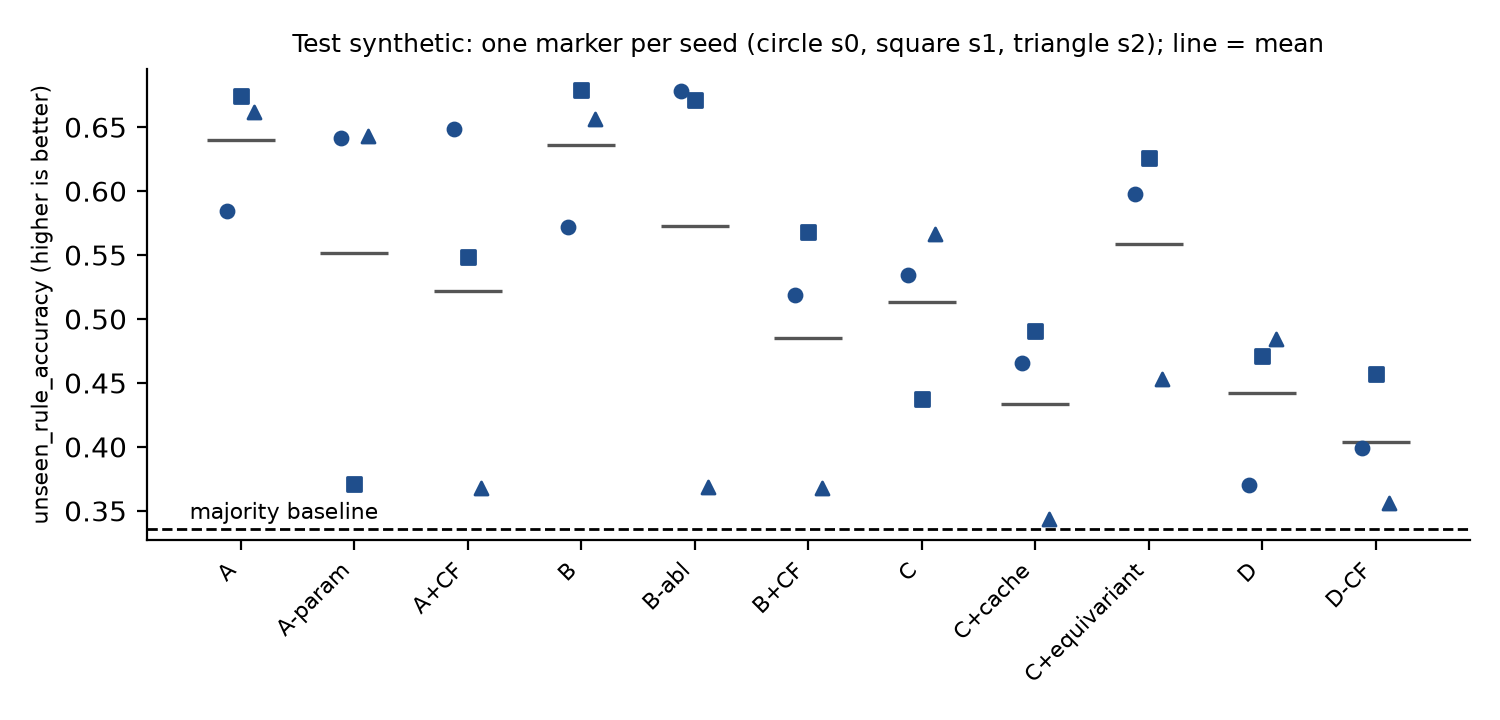
\includegraphics[width=0.9\linewidth]{figures/per_seed.png}
\caption{Test synthetic: \ura{} of each seed (higher is better). The line is the mean over the 3 seeds. The dashed line is the majority baseline ($0.336$). Several models have one seed near the majority baseline.}\label{fig:perseed}
\end{figure}

\paragraph{ProofWriter test sets.}
Table~\ref{tab:pw} gives the accuracy on the three held-out ProofWriter sets next to the test synthetic set.
On \texttt{depth5} and \texttt{birds\_electricity}, several models have a CI above 0 against A.
By the Step 0 rule, these are reliable differences.
We do not read them as evidence for the hypothesis, for three reasons.
First, the seed spread is larger than most differences (for example, \texttt{birds\_electricity}: A $0.552 \pm 0.134$, B $0.666 \pm 0.225$, C+cache $0.587 \pm 0.301$), and the CI does not cover it.
Second, A itself is below the majority baseline on both sets.
Third, only B+CF ($0.763$) and D ($0.771$) are above the \texttt{birds\_electricity} majority baseline ($0.748$), by at most $0.023$.
On \texttt{depth5}, B, C, C+equivariant, and A-param are $0.014$ to $0.023$ above the majority baseline ($0.429$), and the other 7 models are below it.
On \texttt{pararules}, all models are at the majority baseline ($0.455$ to $0.511$ against $0.500$).
We did not compare these accuracies with a published number.
The models do not transfer from the synthetic generator to the ProofWriter text.
The sentence frames and names of \texttt{depth5} occur in the Ettin pretraining data, so \texttt{depth5} results are possibly affected for all models.

\begin{table}[t]
\centering
\caption{Accuracy on the test sets, mean $\pm$ std over 3 seeds (higher is better in all columns). $^{+}$: the CI of the difference to A is above 0. $^{-}$: below 0. No mark: the CI includes 0. The row ``majority'' is the majority baseline.}\label{tab:pw}
\small
\setlength{\tabcolsep}{4pt}
\begin{tabular}{l c c c c}
\toprule
Model & synthetic & \texttt{depth5} & \texttt{birds\_electricity} & \texttt{pararules} \\
\midrule
$n$ & 10{,}086 & 18{,}857 & 5{,}270 & 8{,}008 \\
majority & 0.336 & 0.429 & 0.748 & 0.500 \\
\midrule
\M{A}             & \ms{0.640}{0.049} & \ms{0.406}{0.091} & \ms{0.552}{0.134} & \ms{0.509}{0.004} \\
\M{A-param}       & \ms{0.552}{0.156}\dn & \ms{0.443}{0.058}\up & \ms{0.705}{0.056}\up & \ms{0.489}{0.026}\dn \\
\M{A+CF}          & \ms{0.522}{0.142}\dn & \ms{0.391}{0.039}\dn & \ms{0.548}{0.303} & \ms{0.509}{0.042} \\
\M{B}             & \ms{0.636}{0.056} & \ms{0.452}{0.005}\up & \ms{0.666}{0.225}\up & \ms{0.503}{0.003}\dn \\
\M{B-abl}         & \ms{0.573}{0.177}\dn & \ms{0.384}{0.065}\dn & \ms{0.673}{0.078}\up & \ms{0.503}{0.022}\dn \\
\M{B+CF}          & \ms{0.485}{0.104}\dn & \ms{0.402}{0.090} & \ms{0.763}{0.016}\up & \ms{0.499}{0.012}\dn \\
\M{C}             & \ms{0.513}{0.068}\dn & \ms{0.447}{0.033}\up & \ms{0.669}{0.191}\up & \ms{0.508}{0.014} \\
\M{C+cache}       & \ms{0.433}{0.079}\dn & \ms{0.421}{0.024}\up & \ms{0.587}{0.301}\up & \ms{0.455}{0.102}\dn \\
\M{C+equivariant} & \ms{0.559}{0.092}\dn & \ms{0.449}{0.033}\up & \ms{0.681}{0.040}\up & \ms{0.511}{0.012} \\
\M{D}             & \ms{0.442}{0.062}\dn & \ms{0.368}{0.086}\dn & \ms{0.771}{0.024}\up & \ms{0.498}{0.033}\dn \\
\M{D-CF}          & \ms{0.404}{0.051}\dn & \ms{0.343}{0.040}\dn & \ms{0.410}{0.228}\dn & \ms{0.494}{0.011}\dn \\
\bottomrule
\end{tabular}
\end{table}

\paragraph{External benchmarks.}
Table~\ref{tab:ext} gives the accuracy on the three external benchmarks.
On BoardgameQA, all models have accuracies from $0.362$ to $0.374$ against a majority baseline of $0.367$ (at most $0.006$ above it), and the mean accuracy of each of the 15 subsets is within $0.024$ of its majority baseline (we computed no per-subset CI).
On Super-NaturalInstructions, the accuracies are $0.433$ to $0.443$ against $0.442$ (at most $0.001$ above it), and no difference to A is reliable.
The value $0.442$ is the majority baseline of the pooled set, as the mean of the per-task majority baselines.
So on these two benchmarks no model is clearly above the majority baseline (Figure~\ref{fig:accuracy}).
On DynaBench, A+CF, C, and B-abl are reliably above A ($+0.047$, $+0.036$, $+0.030$).
The highest model on DynaBench (A+CF, $0.546$) is $0.037$ above the majority baseline, and A is $0.010$ below it.
The seed spread is large (A+CF std $0.067$), and the set has 543 records.
So we do not read these differences as a transfer.

\begin{table}[t]
\centering
\caption{Accuracy on the external benchmarks, mean $\pm$ std over 3 seeds (higher is better in all columns). Marks as in Table~\ref{tab:pw}.}\label{tab:ext}
\small
\setlength{\tabcolsep}{4pt}
\begin{tabular}{l c c c}
\toprule
Model & BoardgameQA & DynaBench & Super-NaturalInstructions \\
\midrule
$n$ & 15{,}000 & 543 & 4{,}100 \\
majority & 0.367 & 0.508 & 0.442 \\
\midrule
\M{A}             & \ms{0.373}{0.005} & \ms{0.499}{0.030} & \ms{0.440}{0.007} \\
\M{A-param}       & \ms{0.374}{0.008} & \ms{0.495}{0.092} & \ms{0.435}{0.002} \\
\M{A+CF}          & \ms{0.362}{0.012}\dn & \ms{0.546}{0.067}\up & \ms{0.436}{0.003} \\
\M{B}             & \ms{0.367}{0.000}\dn & \ms{0.475}{0.014} & \ms{0.434}{0.000} \\
\M{B-abl}         & \ms{0.366}{0.004}\dn & \ms{0.529}{0.032}\up & \ms{0.437}{0.002} \\
\M{B+CF}          & \ms{0.367}{0.005}\dn & \ms{0.467}{0.024}\dn & \ms{0.442}{0.004} \\
\M{C}             & \ms{0.368}{0.001}\dn & \ms{0.534}{0.049}\up & \ms{0.441}{0.005} \\
\M{C+cache}       & \ms{0.370}{0.004} & \ms{0.514}{0.011} & \ms{0.442}{0.003} \\
\M{C+equivariant} & \ms{0.368}{0.002}\dn & \ms{0.496}{0.022} & \ms{0.441}{0.003} \\
\M{D}             & \ms{0.368}{0.004}\dn & \ms{0.510}{0.024} & \ms{0.433}{0.006} \\
\M{D-CF}          & \ms{0.369}{0.004} & \ms{0.479}{0.055} & \ms{0.443}{0.002} \\
\bottomrule
\end{tabular}
\end{table}

\begin{figure}[t]
\centering
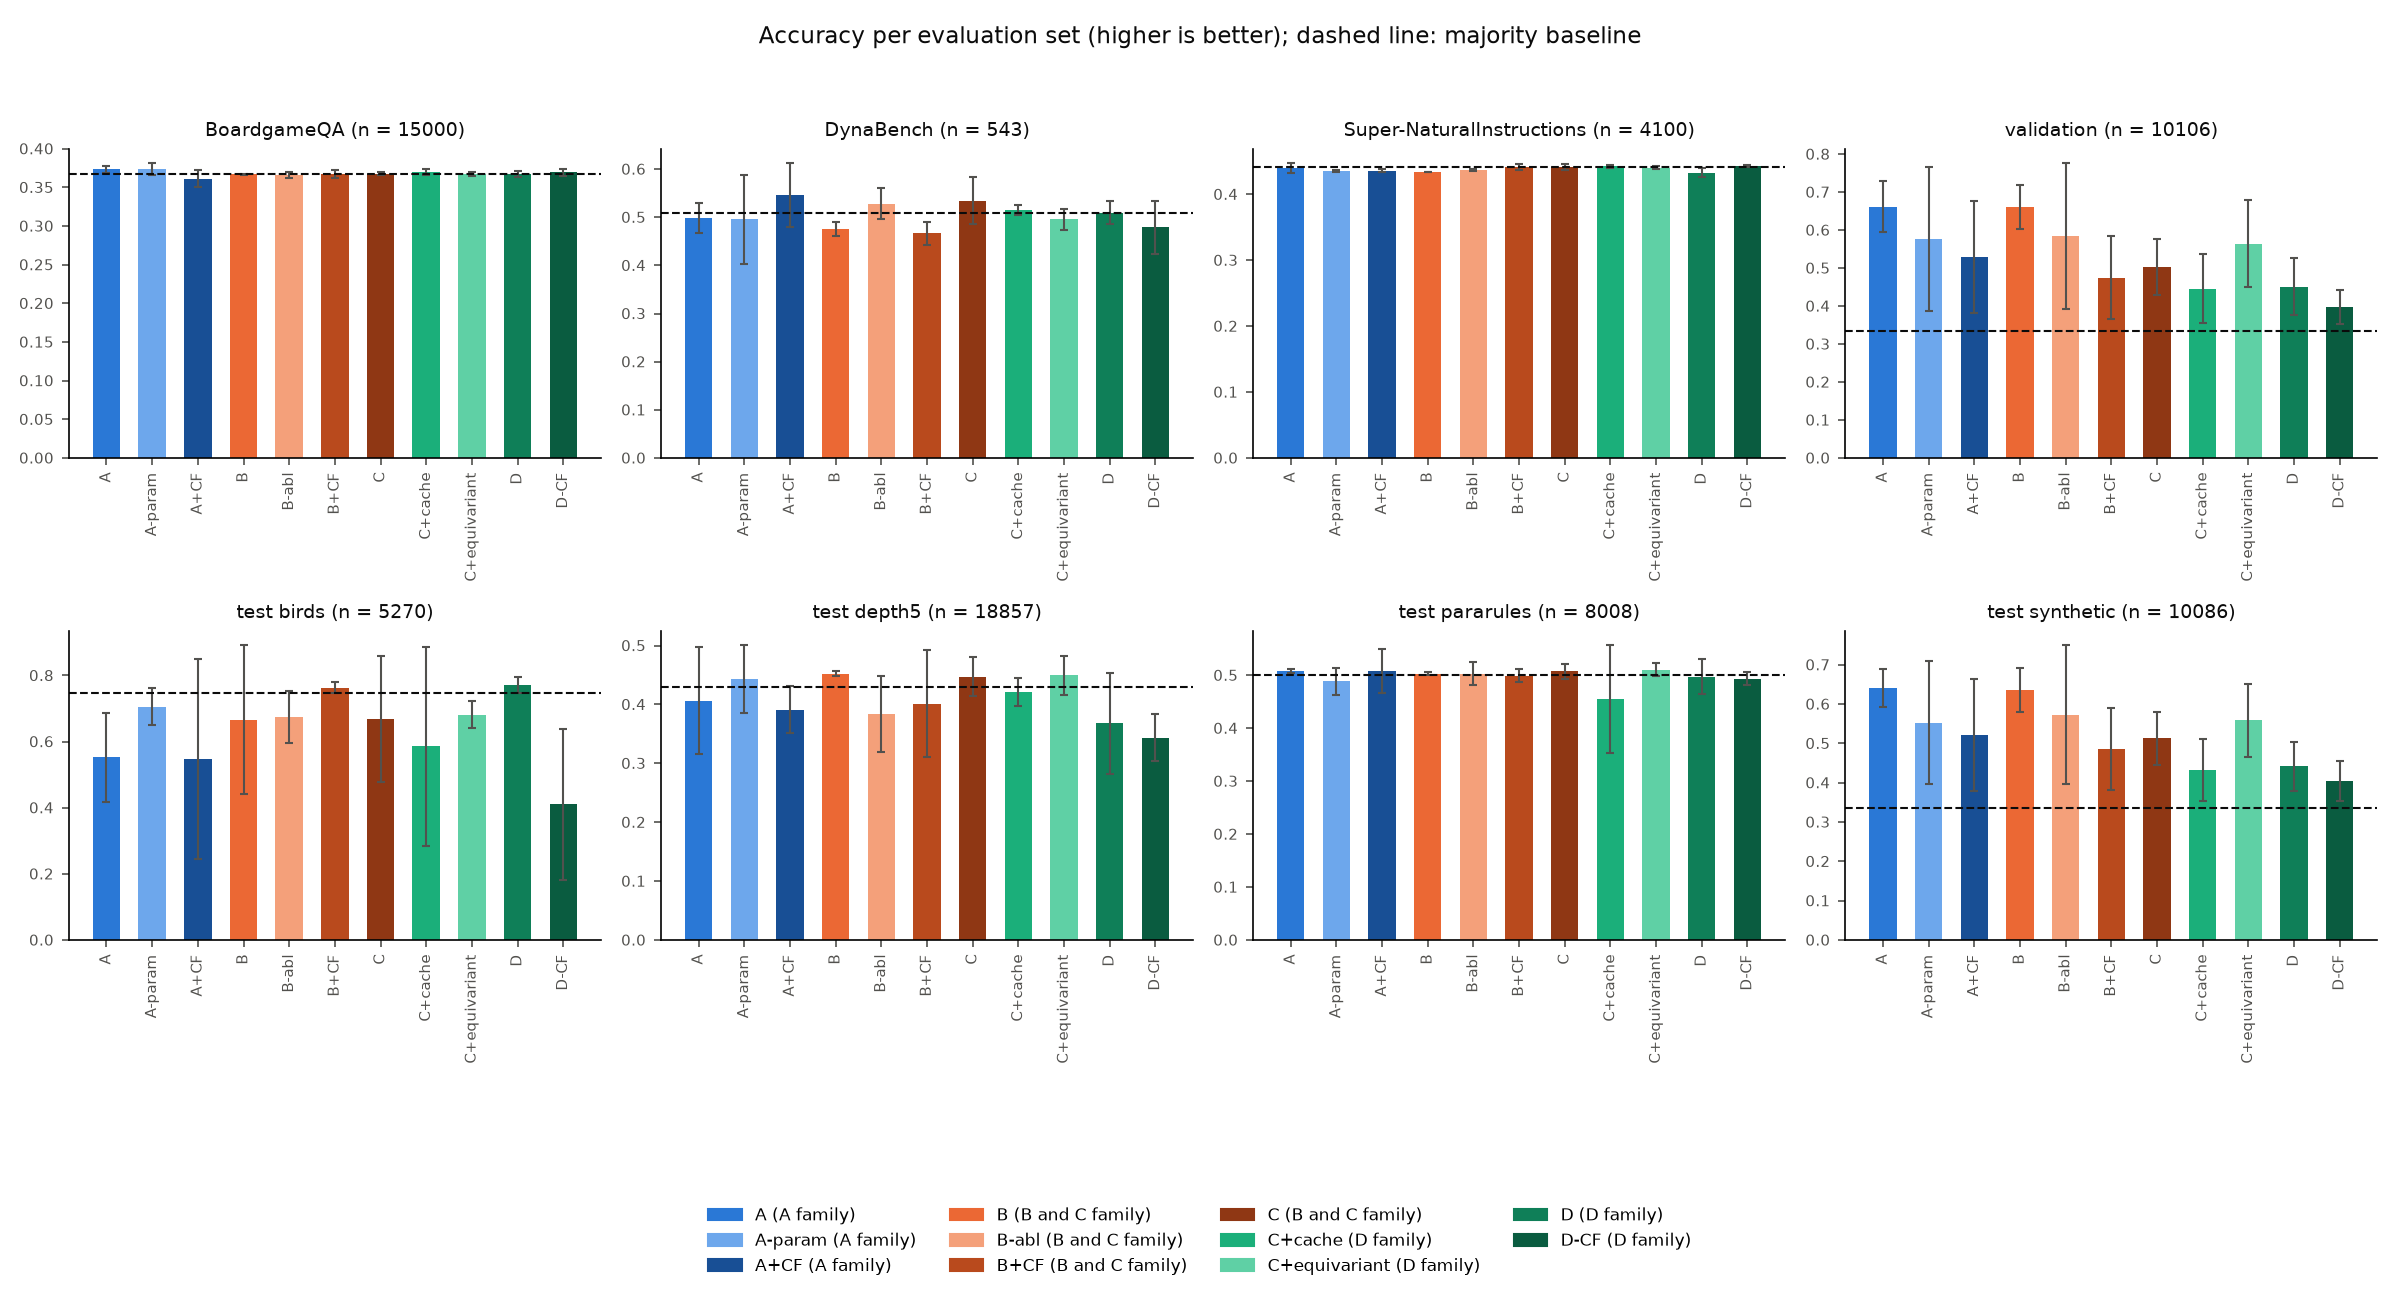
\includegraphics[width=\linewidth]{figures/accuracy.png}
\caption{Accuracy on all evaluation sets (higher is better). Bars show the mean over 3 seeds, error bars show the standard deviation over seeds, and the dashed line is the majority baseline.}\label{fig:accuracy}
\end{figure}

\paragraph{Against the Step 0 criteria.}
The success criterion asks for a reliable improvement over A in held-out rule generalization and in counterfactual decision accuracy.
On test synthetic, which is the set with unseen rules, no model meets it on either metric.
On \cpa{}, every model is reliably lower than A.
The reliable gains on two ProofWriter sets and on DynaBench do not meet the intent of the criterion (see above), and no model has a reliable gain on both primary metrics.
We therefore conclude that the criterion is not met.

\subsection{Counterfactual pairs by edit type and depth}

Table~\ref{tab:edit} gives \cpa{} for each edit type and original label on test synthetic.
We show only the cells with at least 40 pairs.
\texttt{exception\_remove} (69 pairs) and \texttt{priority\_swap} (53 pairs) are too few to report by type.
Among the six models in the table, A is the highest or within $0.02$ of the highest in 16 of the 19 single cells.
The cells for \texttt{threshold\_shift} and \texttt{fact\_number} are low for all models (at most $0.259$).
The largest advantage of B over A is in the cell \texttt{condition\_negate} / multi\_choice ($0.331$ against $0.231$).
The cells have no CI, and the numbers are means over 3 seeds with a large seed spread.
Figure~\ref{fig:paired} shows \cpa{} on validation and test synthetic.
Table~\ref{tab:depth} gives the accuracy of the \texttt{depth5} set by question depth.
The per-depth majority baseline is not computed, so the rise from depth 0 to depth 5 has no reference.

\begin{table}[t]
\centering
\caption{Test synthetic, \cpa{} per edit type and original label, mean over 3 seeds (higher is better in all columns). $n$ is the number of pairs. The ranges for \texttt{fact\_number} (True, False, Unknown) cover 46 to 54 pairs per cell.}\label{tab:edit}
\scriptsize
\setlength{\tabcolsep}{4pt}
\resizebox{\linewidth}{!}{%
\begin{tabular}{l r c c c c c c}
\toprule
Edit type / original label & $n$ & \M{A} & \M{B} & \M{C} & \M{C+equivariant} & \M{D} & \M{D-CF} \\
\midrule
\texttt{fact\_flip} / True        & 211 & 0.796 & 0.776 & 0.675 & 0.719 & 0.425 & 0.359 \\
\texttt{fact\_flip} / False       & 218 & 0.742 & 0.708 & 0.602 & 0.680 & 0.430 & 0.381 \\
\texttt{fact\_flip} / Unknown     & 69  & 0.787 & 0.739 & 0.614 & 0.652 & 0.517 & 0.420 \\
\texttt{fact\_flip} / multi\_choice & 862 & 0.616 & 0.610 & 0.376 & 0.456 & 0.225 & 0.166 \\
\texttt{fact\_remove} / True      & 345 & 0.705 & 0.719 & 0.559 & 0.629 & 0.397 & 0.299 \\
\texttt{fact\_remove} / False     & 375 & 0.730 & 0.689 & 0.591 & 0.645 & 0.404 & 0.327 \\
\texttt{fact\_remove} / Unknown   & 107 & 0.604 & 0.567 & 0.539 & 0.564 & 0.505 & 0.402 \\
\texttt{fact\_remove} / multi\_choice & 193 & 0.389 & 0.361 & 0.197 & 0.278 & 0.140 & 0.114 \\
\texttt{condition\_negate} / True & 345 & 0.351 & 0.338 & 0.135 & 0.200 & 0.097 & 0.100 \\
\texttt{condition\_negate} / False & 312 & 0.366 & 0.347 & 0.151 & 0.262 & 0.104 & 0.136 \\
\texttt{condition\_negate} / Unknown & 636 & 0.525 & 0.529 & 0.316 & 0.398 & 0.279 & 0.172 \\
\texttt{condition\_negate} / multi\_choice & 166 & 0.231 & 0.331 & 0.183 & 0.235 & 0.145 & 0.153 \\
\texttt{rule\_remove} / True      & 98  & 0.361 & 0.344 & 0.143 & 0.197 & 0.088 & 0.156 \\
\texttt{rule\_remove} / False     & 106 & 0.292 & 0.343 & 0.164 & 0.252 & 0.091 & 0.154 \\
\texttt{rule\_remove} / multi\_choice & 48 & 0.299 & 0.285 & 0.229 & 0.222 & 0.139 & 0.215 \\
\texttt{threshold\_shift} / True  & 157 & 0.176 & 0.146 & 0.146 & 0.119 & 0.138 & 0.149 \\
\texttt{threshold\_shift} / False & 163 & 0.200 & 0.149 & 0.117 & 0.149 & 0.119 & 0.170 \\
\texttt{threshold\_shift} / Unknown & 98 & 0.211 & 0.241 & 0.235 & 0.211 & 0.259 & 0.156 \\
\texttt{fact\_number} / multi\_choice & 236 & 0.168 & 0.134 & 0.113 & 0.129 & 0.123 & 0.114 \\
\texttt{fact\_number} / True, False, Unknown & 46--54 & 0.135--0.203 & 0.111--0.206 & 0.058--0.191 & 0.086--0.156 & 0.130--0.177 & 0.057--0.136 \\
\bottomrule
\end{tabular}}
\end{table}

\begin{table}[t]
\centering
\caption{ProofWriter \texttt{depth5}, accuracy per question depth, mean over 3 seeds (higher is better in all columns). The majority baseline of the whole set is $0.429$. The per-depth majority baseline is not computed. Depths 6 and 7 have 10 questions, which are too few to report.}\label{tab:depth}
\small
\setlength{\tabcolsep}{4pt}
\begin{tabular}{l r c c c c c c c}
\toprule
Depth & $n$ & \M{A} & \M{A-param} & \M{B} & \M{C} & \M{C+equivariant} & \M{D} & \M{D-CF} \\
\midrule
0 & 5{,}774 & 0.355 & 0.364 & 0.402 & 0.360 & 0.388 & 0.404 & 0.264 \\
1 & 4{,}247 & 0.343 & 0.389 & 0.381 & 0.376 & 0.391 & 0.351 & 0.278 \\
2 & 2{,}730 & 0.431 & 0.464 & 0.478 & 0.480 & 0.479 & 0.355 & 0.376 \\
3 & 2{,}249 & 0.467 & 0.535 & 0.535 & 0.544 & 0.528 & 0.352 & 0.426 \\
4 & 1{,}990 & 0.495 & 0.556 & 0.544 & 0.574 & 0.543 & 0.346 & 0.458 \\
5 & 1{,}857 & 0.507 & 0.550 & 0.536 & 0.579 & 0.536 & 0.354 & 0.470 \\
\bottomrule
\end{tabular}
\end{table}

\begin{figure}[t]
\centering
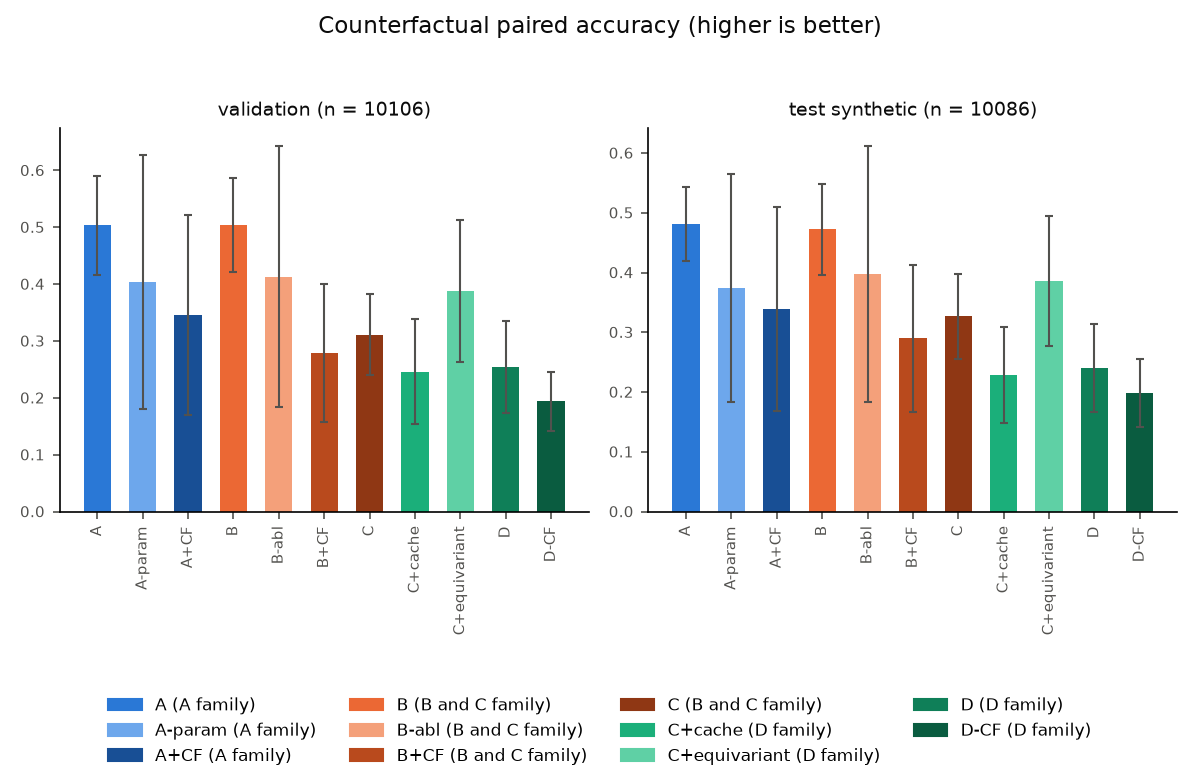
\includegraphics[width=0.95\linewidth]{figures/paired_accuracy.png}
\caption{\cpa{} on validation and on test synthetic (higher is better). Bars show the mean over 3 seeds, and error bars show the standard deviation over seeds.}\label{fig:paired}
\end{figure}

\subsection{Option-order invariance}

On validation, the argmax agreement under a fixed random permutation of the options is $1.000$ (to three decimals) for all runs.
In the Step 7 check, 8{,}407 to 8{,}422 of the 10{,}106 records change their option order, depending on the seed, and the mean absolute probability difference per run is at most $1.1 \times 10^{-6}$.
The shuffled-order \ura{} differs from the canonical-order value by at most $0.0011$.
A, B, and C score each option alone, so they are order-invariant by construction.
The block of D adds an interaction between options and keeps the invariance.
Thus this metric does not separate D from the other models.
On the test split, the mean argmax agreement is $0.993$ to $1.000$ for each model and subset.
The lowest value is C+cache on \texttt{birds\_electricity} ($0.993 \pm 0.012$).
We did not examine why the agreement on test is $0.993$ to $1.000$ and not $1.000$ (fp16 on the L4, or near-tied scores on longer inputs).

\subsection{Calibration}

No model has the lowest ECE on all sets (Figure~\ref{fig:ece}).
On test synthetic, C+cache has the lowest ECE ($0.036$), and A has $0.075$ (Table~\ref{tab:testsyn}).
On validation, C+cache also has the lowest ECE ($0.024$).
C+cache has a low accuracy on both sets, so a low ECE does not make it a better decision model.
ECE varies between seeds and between sets: for example, D has an ECE of $0.323$ on \texttt{birds\_electricity}.
We do not draw a conclusion about calibration beyond this.

\begin{figure}[t]
\centering
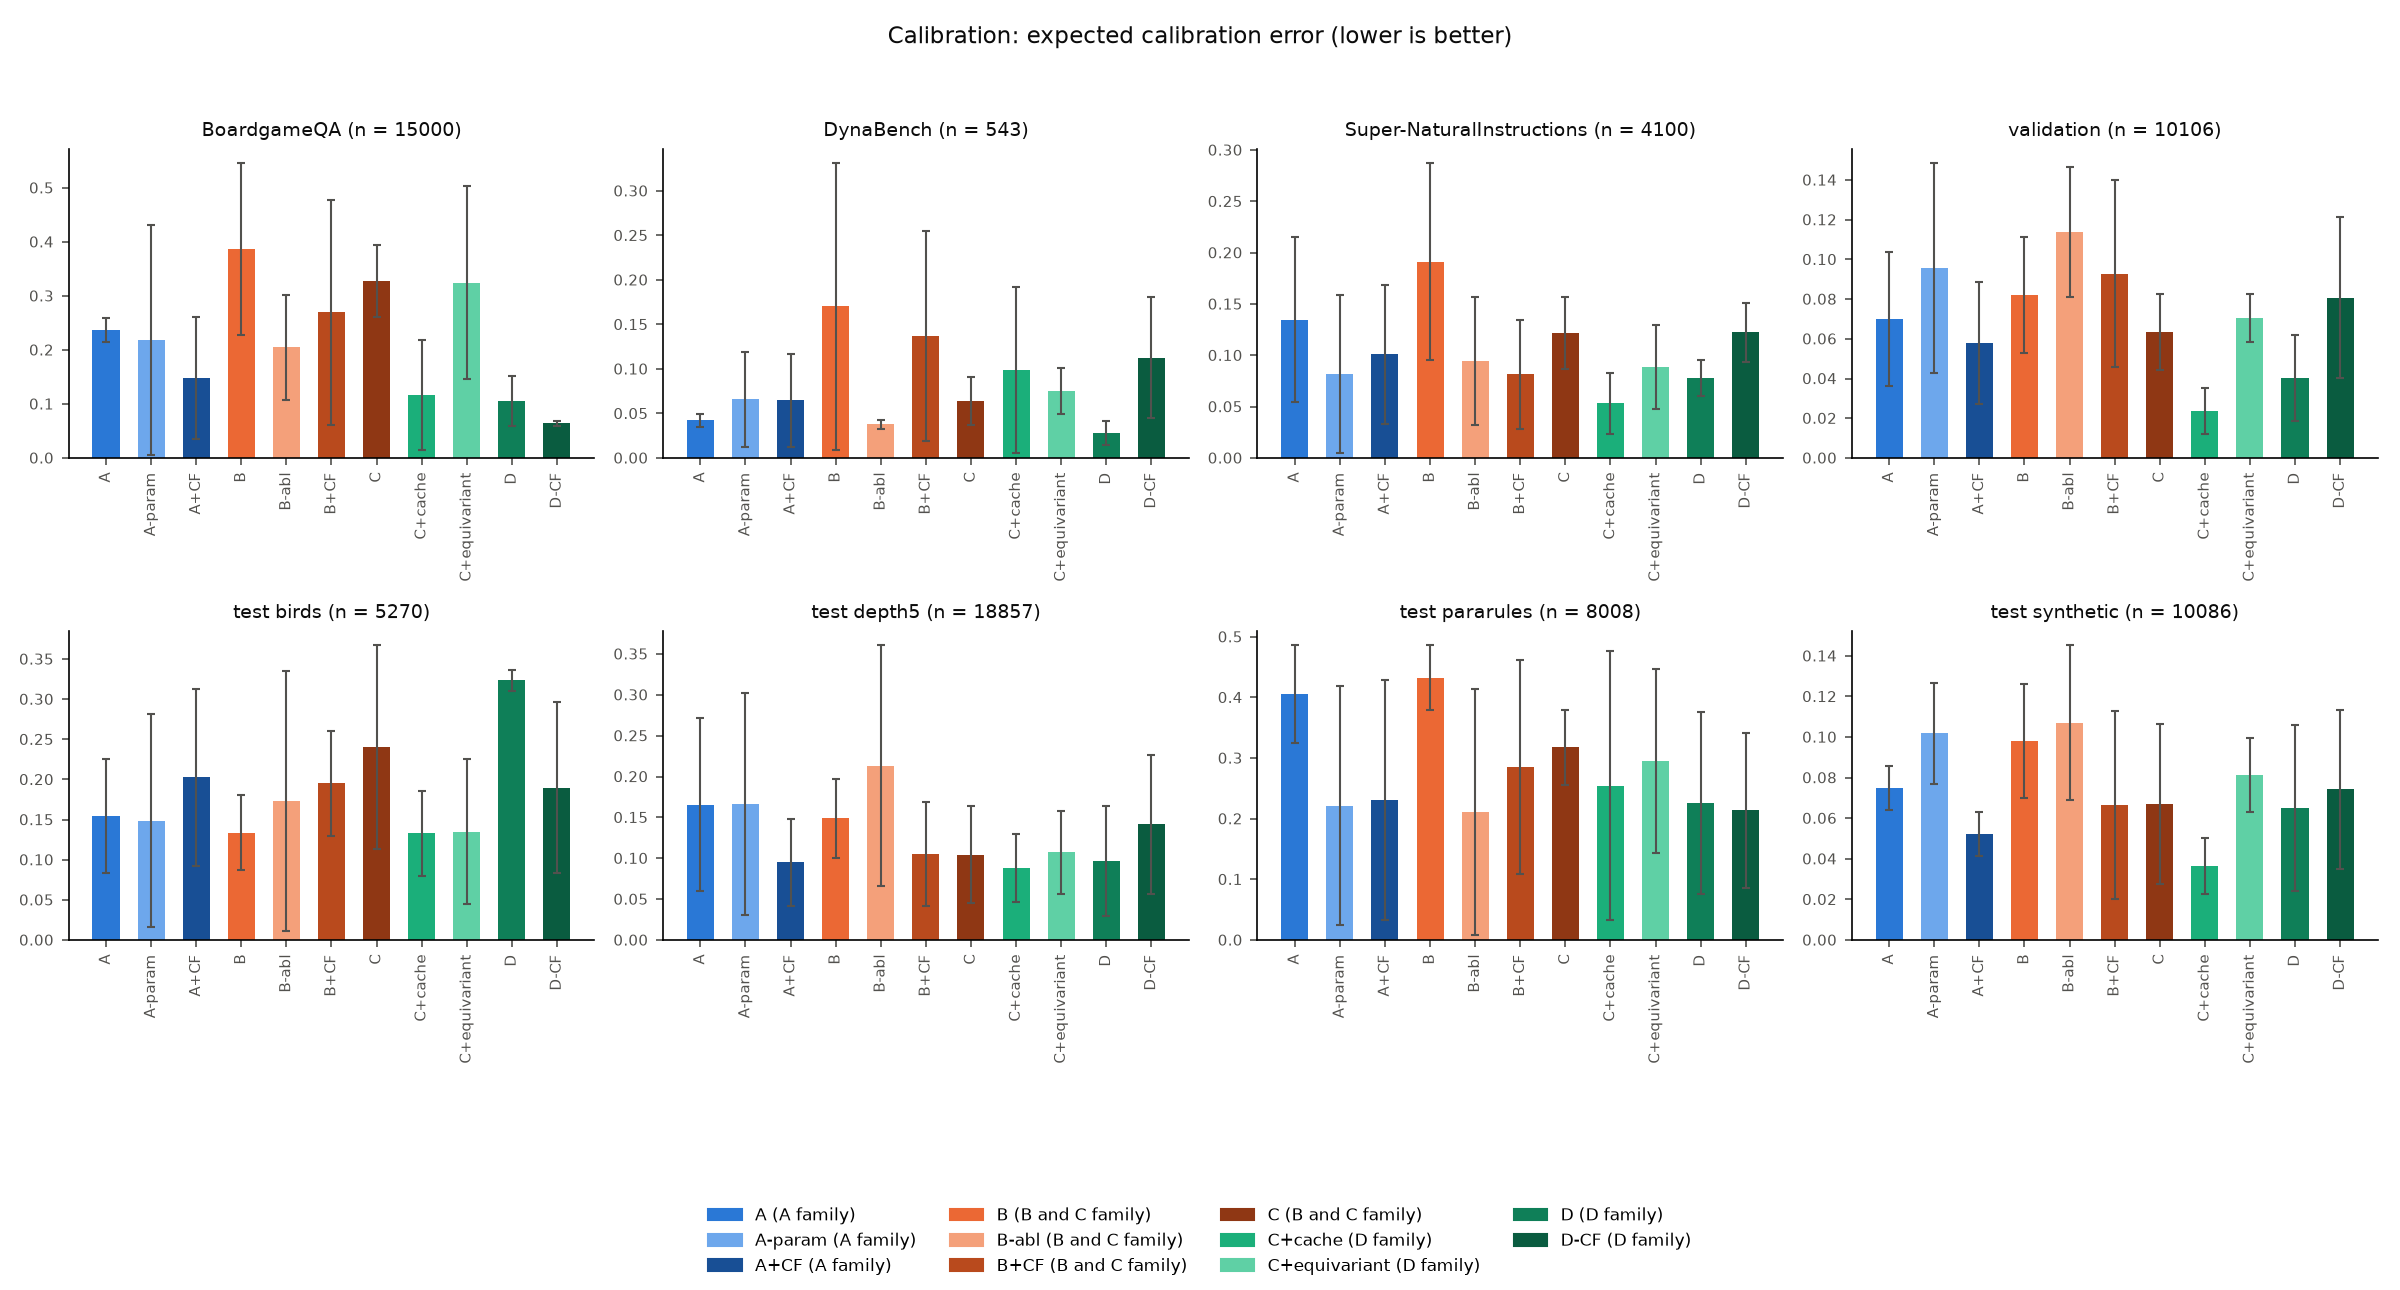
\includegraphics[width=\linewidth]{figures/ece.png}
\caption{Expected calibration error on all evaluation sets (lower is better). Bars show the mean over 3 seeds, and error bars show the standard deviation over seeds.}\label{fig:ece}
\end{figure}

\subsection{Latency, memory, and cache}

Table~\ref{tab:eff} gives the efficiency measurements.
All values are from an NVIDIA L4 GPU (Colab) at batch size 1 with fp16 and forward passes only, as the mean over 3 seeds.
Figure~\ref{fig:latency} shows latency against accuracy.
We have no measurement on a mobile device (Section~\ref{sec:deviations}).

A is the fastest model (p50 9.53 ms), and it has the highest mean \ura{} on test synthetic (for B, the CI of the difference includes 0).
The models with the split encoding need about 2 times the latency of A without a cache (D: 19.80 ms).
The probable reason is that the bottom layers run on 3 sequences for each record, and the batch-size-1 time on the L4 is mostly kernel launch time (we did not test this).
With the state and the instruction cached, D needs 11.76 ms.
This is still 9\% more than C (10.78 ms), because only 3 of 7 layers are cached: the top 4 layers run on the full concatenation for each option.
So the cache does not reduce the latency at batch size 1 below the latency of C or A.
A smaller $J$ would cache more layers, but the split encoding already costs accuracy at $J = 4$.
The peak CUDA memory at batch size 1 is within 0.5 MB for the joint and the split encoding (one joint model, C+equivariant: 39.3 MB; split models: 39.5 to 39.8 MB above the model).
The cache needs 37.3 KB per state (72.8 tokens on average) and 100.1 KB per instruction (195.5 tokens), in fp16, as the mean over the distinct validation items.
Validation has 10{,}106 records, 5{,}642 distinct states (1.79 records per state), and 6{,}728 distinct instructions.
The batch-evaluation latency per record is not comparable between the joint and the split models, because the evaluation budget does not count the top-layer tokens of the split models.

\begin{table}[t]
\centering
\caption{Latency and memory on the L4 at batch size 1, mean over 3 seeds. All columns: lower is better. ``n/a'': no value exists for the model. ``n.m.'': not measured (the source holds no value). ``Peak MB'' is the peak CUDA memory above the model. ``Both cached'' means that the state and the instruction are cached.}\label{tab:eff}
\footnotesize
\setlength{\tabcolsep}{3pt}
\begin{tabular}{l r *{4}{>{\raggedleft\arraybackslash}p{1.45cm}} r r}
\toprule
Model & Params & p50 ms, no cache & p95 ms, no cache & p50 ms, state cached & p50 ms, both cached & Model MB, fp16 & Peak MB \\
\midrule
\M{A}             & 16{,}863{,}745 & 9.53  & 10.59 & n/a   & n/a   & 33.73 & n.m. \\
\M{A-param}       & 17{,}146{,}625 & 14.37 & 15.30 & n/a   & n/a   & n.m.  & n.m. \\
\M{A+CF}          & 16{,}863{,}745 & 9.81  & 11.21 & n/a   & n/a   & n.m.  & n.m. \\
\M{B}             & 17{,}146{,}945 & 10.68 & 11.90 & n/a   & n/a   & 34.29 & n.m. \\
\M{B-abl}         & 18{,}744{,}385 & 11.93 & 12.71 & n/a   & n/a   & n.m.  & n.m. \\
\M{B+CF}          & 17{,}146{,}945 & 10.92 & 11.79 & n/a   & n/a   & n.m.  & n.m. \\
\M{C}             & 17{,}146{,}945 & 10.78 & 11.44 & n/a   & n/a   & 34.29 & n.m. \\
\M{C+cache}       & 17{,}146{,}945 & 19.98 & 21.78 & 15.46 & 11.51 & 34.29 & 39.8 \\
\M{C+equivariant} & 17{,}410{,}625 & 11.12 & 12.79 & n/a   & n/a   & 34.82 & 39.3 \\
\M{D}             & 17{,}410{,}625 & 19.80 & 21.94 & 15.67 & 11.76 & 34.82 & 39.8 \\
\M{D-CF}          & 17{,}410{,}625 & 20.25 & 22.03 & 16.04 & 12.06 & 34.82 & 39.5 \\
\bottomrule
\end{tabular}
\end{table}

\begin{figure}[t]
\centering
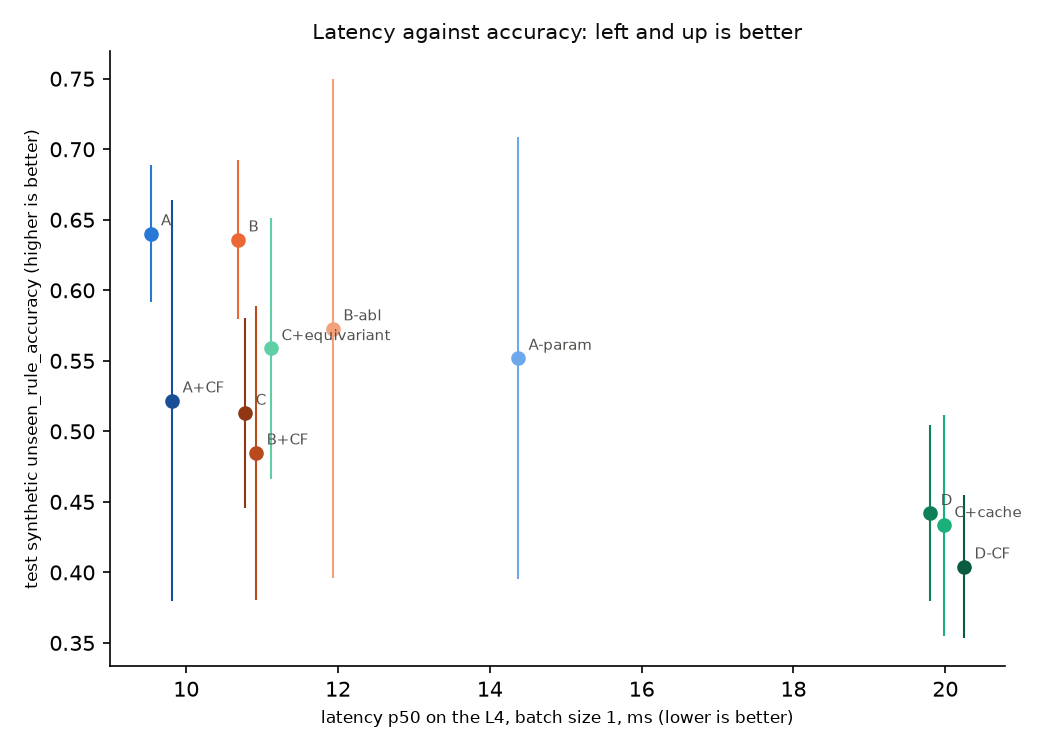
\includegraphics[width=0.8\linewidth]{figures/latency_accuracy.png}
\caption{Latency at batch size 1 on the L4 (p50, lower is better) against \ura{} on test synthetic (higher is better). Error bars show the standard deviation over seeds. A is in the top left corner.}\label{fig:latency}
\end{figure}

% =====================================================================
\section{Discussion}\label{sec:discussion}

\paragraph{What the data show.}
At a budget of 12{,}000 steps, one trial, and 3 seeds, no architecture beats the plain Ettin-17M baseline on unseen rules.
B equals A on \ura{} (the CI includes 0) and is $0.009$ lower on \cpa{} (the CI is below 0).
The hypernetwork head gives no gain, and it costs 12\% more latency (10.68 ms against 9.53 ms).
The controls explain the other results.
A+CF and B+CF show that our form of CF batches decreases the accuracy without any architecture change.
A-param shows that the extra parameters alone do not help either, and B-abl and A-param have similar means ($0.584$ and $0.576$; no CI computed).
C+cache and D show that the split encoding costs accuracy.
The contrast C+equivariant $-$ C ($+0.061$; weak evidence, 2 of 3 seed pairs) shows a gain from the set-attention block with the joint encoding.
The contrast D $-$ C+cache ($+0.006$) shows no reliable effect of the block on \ura{} with the split encoding.
The contrast D $-$ D-CF ($+0.054$; weak evidence, 2 of 3 seed pairs) shows a gain from CF with the consistency loss inside D, but D stays far below A.

\paragraph{Possible reasons (not tested).}
We offer these reasons as hypotheses.
We did not test them.
(1) B receives $z$ from the same encoder pass that already reads the instruction jointly with the state, so the hypernetwork gets no information that A does not already have.
(2) CF batches hold about 11 units, not 32 almost independent records, so each update has less variety, and the runs leave chance later.
(3) The split encoding removes the cross-attention between state, instruction, and option in 3 of 7 layers, and the pretraining did not give the top layers the positions and the three \texttt{[CLS]}/\texttt{[SEP]} pairs of the split input.
For the CF runs and the D runs, the best checkpoint is often at step 11{,}000 or 12{,}000, so the curves still rise at the end of training.
A longer run, a mix of paired and random batches, or a learning-rate search could change the result.
We did not run these, because they need the same extra budget for all models.

\paragraph{Training reliability.}
Several models have one of 3 seeds near chance (Figure~\ref{fig:perseed}).
This is the case for A-param, A+CF, B-abl, B+CF, C+cache, D, and D-CF (the lowest seed of each is $0.343$ to $0.367$ on validation, against a majority baseline of $0.333$), and it makes the std and the CI-based marks less informative.
The bootstrap CI covers the record sample, so the CI is narrow even when the seed spread is wide.
Our conclusions rely on the sign and the consistency of a difference over validation and test more than on a single CI.

\paragraph{No transfer to natural text.}
All models train on synthetic text only.
On ProofWriter \texttt{pararules}, BoardgameQA, DynaBench, and Super-NaturalInstructions, the models are at the majority baseline.
So the synthetic training gives no measurable transfer to natural-language rules at this size and budget.
The success criterion does not require such a transfer, but a mobile decision model needs it in practice.

\paragraph{What the data do not show.}
The data do not show that rule conditioning, counterfactual learning, or cacheable scoring cannot help.
They show that, in these implementations and at this budget, no gain exists that the controls and the seed spread allow us to separate from zero.
We make no claim about larger models, longer training, other forms of counterfactual training, or other conditioning methods.

% =====================================================================
\section{Limitations}\label{sec:limits}

\begin{itemize}
  \item \textbf{Seeds, trials, steps.} We use 3 seeds, one hyperparameter trial, and 12{,}000 steps for every model. The bootstrap CI covers the record sample only, not the seed variance. On the ProofWriter sets, the seed spread is larger than most differences.
  \item \textbf{Fixed design choices.} The consistency weight (1.0), the rank (8), the hypernetwork width (64), the number of joint layers ($J = 4$), and the form of CF batches are fixed choices. We did not search them.
  \item \textbf{No external baselines.} We did not evaluate fine-tuned Ettin-32M and DeBERTa-v3-xsmall. So we have no comparison with a model with different pretraining. We did not evaluate Jev.
  \item \textbf{Shared initialization and contamination.} All 11 models share the Ettin-17M initialization, so a contamination affects them equally. The sentence frames and names of \texttt{depth5} occur in the Ettin pretraining data (maximum 8-gram share $0.10$ for a kept record). Super-NaturalInstructions is not scanned, and it is possibly seen in pretraining. We did not check web-crawl sources for BoardgameQA and DynaBench.
  \item \textbf{DynaBench size.} DynaBench has 543 records, so its CIs are wide.
  \item \textbf{Open-world ProofWriter only.} The ProofWriter test sets are open-world (True, False, Unknown). They are comparable only with published open-world results, not with the closed-world RuleTaker results.
  \item \textbf{No per-depth majority baseline} for \texttt{depth5}, and depths 6 and 7 have 10 questions.
  \item \textbf{Multi-choice rule-edit pairs.} Validation has such units only in composition \texttt{c23} (31 units). On test, the numbers of multi-choice rule-edit pairs are \texttt{condition\_negate} 166, \texttt{rule\_remove} 48, \texttt{threshold\_shift} 26, \texttt{priority\_swap} 2, and \texttt{exception\_remove} 0. The split per test composition (\texttt{c18}, \texttt{c28}, \texttt{c31}) is not computed.
  \item \textbf{Synthetic data only.} The labels are correct by construction, but the language has 15 templates and 12 vocabulary pools. The results may not hold for other rule languages.
  \item \textbf{Validation selection.} The checkpoint selection uses validation, so validation numbers are slightly optimistic.
  \item \textbf{Option-order invariance.} The metric does not separate the models on validation, and we did not examine why the test agreement is $0.993$ to $1.000$ and not $1.000$.
  \item \textbf{Efficiency data.} All latency and memory values are from one L4 GPU at batch size 1. We have no CPU, mobile, or INT8 value. The peak memory of A, B, and C is not measured, because their order-invariance check ran on the CPU.
  \item \textbf{Software versions.} The Step 6 runs used torch 2.11.0 and transformers 5.18.0. The Step 7 and Step 8 runs used transformers 5.20.1. The versions of the Step 5 runs are not recorded. The validation values on the CPU (fp32) differ from the L4 (fp16) by at most $0.0016$ on a sample of 1{,}906 records.
\end{itemize}

% =====================================================================
\section{Deviations from the Pre-Registration}\label{sec:deviations}

We list every deviation from \texttt{configs/protocol.yaml} and \texttt{steps.md}.
\begin{enumerate}
  \item \textbf{External baselines not evaluated.} The protocol names fine-tuned Ettin-32M and DeBERTa-v3-xsmall. We evaluated the 33 existing runs only (the minimum scope, a scope decision of the project owner). The code and the configurations for the baselines exist, so they can run later.
  \item \textbf{Jev not evaluated.} The protocol allows Jev only through API access, and we have no API access.
  \item \textbf{Mobile measurements not made (Step 9 skipped).} The protocol pre-registered model size, peak RAM, p50 and p95 latency, and the INT8 accuracy loss on the Google Pixel 8 (ONNX Runtime Android). We did not make any of these measurements and we did not export a model to ONNX. The reason is that no architecture is better than A, and the best validation result is A (equal to B), which is the plain Ettin-17M baseline. A mobile benchmark of A measures no CRUX part. The success criterion asks for ``practical mobile inference performance'', and we cannot assess it. We have the parameter counts, the fp16 model size, the peak CUDA memory, and the L4 latency only.
  \item \textbf{One trial instead of a larger search budget.} The protocol gives 6 trials as an example for the equal hyperparameter search budget. The first Step 5 sweep used 6 trials at 6{,}000 steps. We then reduced the budget to one trial (learning rate $3\times10^{-5}$, weight decay $0.01$) at 12{,}000 steps for all models, to pay for Steps 6 and 7 with the available compute credit. This applies equally to all models.
  \item \textbf{Step 5 rerun.} At 6{,}000 steps, 48 of 72 runs had their best checkpoint at the last step, and many seeds left chance only after 2{,}000 to 4{,}000 steps. The seed spread was too large for a fair comparison (for example A: $0.561 \pm 0.192$). We repeated Step 5 with 12{,}000 steps and one trial. The 6{,}000-step runs are not used for any result in this paper. The ranking changed: at 6{,}000 steps, B-abl and A-param were above A ($+0.041$ and $+0.056$) and B was below A ($-0.079$); at 12{,}000 steps, B equals A, and B-abl and A-param are below A. This change was made after seeing the 6{,}000-step results on validation. It is a post-hoc change. It does not use the test split.
  \item \textbf{Earlier search changes in Step 5.} Before any run of trials 1 to 5, we changed two learning rates of the search (trial 1: $2\times10^{-5}$ to $6\times10^{-5}$, trial 5: $2\times10^{-5}$ to $7\times10^{-5}$, weight decay $0.1$ to $0.01$) for all architectures, because the first runs stayed at chance. We restarted all runs with the learning-rate multiplier of new modules set to 1 (not 10) after a diagnosis on A, and 23 runs with multiplier 10 are not used. We fixed an fp16 overflow of B-abl by a soft bound on the generated factors (A, B, and A-param stay bit-identical).
  \item \textbf{Extra control D-CF.} D-CF is not in the pre-registered list. We added it after Step 6 shows that C is worse than B. It separates the effect of both D parts from the effect of CF.
  \item \textbf{Definition of CF.} The protocol requires the same data for all configurations. Thus we define CF as the batch order (whole units in a batch), not as additional counterfactual data (Section~\ref{sec:models}).
  \item \textbf{Test split changed before the freeze.} The contamination scan found 1{,}173 ProofWriter \texttt{depth5} records with an 8-gram share above $0.10$. We removed them by the pre-registered rule, and we froze the test split again (42{,}221 records). No model had seen the test split at that time. An earlier build of Step 4 computed test baselines. We deleted these values, and nothing used them.
  \item \textbf{Generator targets changed after the first runs.} After the first 100{,}000-record runs, we changed some targets of the generator spec (the label balance applies to original records at depth 1 or more; the target share of the edit types \texttt{exception\_remove} and \texttt{priority\_swap}; \texttt{max\_attempts} 200). We also corrected the spec on relevant stays: only 8.5\% of the binary stays and 20.4\% of the multi-choice stays are \texttt{edit\_relevant}, not ``80\% or more''. The labels do not change. The reasons are in \texttt{docs/generator\_spec.md}.
  \item \textbf{Open-world ProofWriter instead of RuleTaker.} The test split has no closed-world RuleTaker set, so the open-world ProofWriter sets stand in for it.
  \item \textbf{Super-NaturalInstructions subset.} We exclude 6 classification tasks with the license ``Unknown'' (of the 16 such tasks among the 119 held-out tasks), and we use 41 tasks with a cap of 100 instances.
  \item \textbf{Evaluation limits in Step 8.} The benchmark run uses larger token limits than training (\texttt{max\_length} 5{,}600), so that no record is truncated. All models use the same limits.
  \item \textbf{GPU type.} The common instruction of the project names a Colab T4 GPU. All runs used an L4 GPU, because it is faster at a similar cost. The T4 was used only for a timing run. The L4 also runs fp16, as the T4.
  \item \textbf{Edits of the protocol file after the freeze.} \texttt{configs/protocol.yaml} changed in four later commits (Steps 4 and 5). The changes include the split sizes and hashes, the training budget of 6{,}000 steps, and the change to 12{,}000 steps and one trial. The seeds, the metrics, and the statistics did not change.
  \item \textbf{Protocol amendment.} The protocol allows one amendment with numeric targets after A is measured. We made no amendment.
\end{enumerate}

% =====================================================================
\section{Reproducibility}\label{sec:repro}

\paragraph{Code and configurations.}
The repository holds the code (\texttt{crux/}), the configurations (\texttt{configs/}), Colab notebooks (\texttt{notebooks/}) for Steps 1, 2, 4, 5, 6, and 7 (the Step 8 evaluation runs with \texttt{crux/colab\_eval.py}), the unit tests (401 tests pass), and the documentation (\texttt{docs/}).
The frozen protocol is \texttt{configs/protocol.yaml}.
The frozen split hashes are in Appendix~\ref{app:hash}, and in \texttt{configs/splits\_manifest.json} and \texttt{configs/protocol.yaml}.
\texttt{load\_split} checks the hash of each split file against the manifest and refuses the test split unless a flag is set.
The generator is deterministic.
Two runs give the same hash for the output files.

\paragraph{Compute.}
All training ran on Colab L4 GPUs with fp16.
The first Step 5 sweep (6{,}000 steps, 72 runs, not used for results) took about 55 compute units.
The 23 runs with the learning-rate multiplier 10 were stopped earlier, and their cost is not recorded.
The other figures omit these two items.
The compute use was about 18 compute units for the Step 5 rerun (12 runs), 14.6 units for Step 6 (9 runs, with a smoke run and 2 repeated runs), 13.0 units for Step 7 (12 runs, with a smoke run), and 3.8 units for the Step 8 evaluation.
Each Step 8 evaluation of one run took about 2.5 to 3 minutes (test: 42{,}221 records in 86 to 105 seconds).

\paragraph{Reproduction check.}
We train A with seed index 0 (seed 13) and D with seed index 0 (seed 13) again from a clean Colab VM at commit \texttt{2d3e4b0}.
The release build of the code is at commit \texttt{a00d586}.
The check compares the new numbers with the numbers of this paper and with the seed spread.
\REPRO{}
Bit-exact equality is not expected, because the runs use fp16 on a GPU and the library versions can differ.
The seed spread of the results in this paper (for example A on validation: $0.589$, $0.720$, $0.675$ for the 3 seeds) sets the scale of a comparison.

\paragraph{Not in the repository.}
The run outputs (\texttt{runs/}) are not in git.
The converters build the processed data (\texttt{data/}) from the official sources.
We do not redistribute Super-NaturalInstructions instances.
The release holds the task identifiers and hashes only.
The code is at \url{https://github.com/0xAnto/crux}.
The trained weights (11 models, 3 seeds each) are at \url{https://huggingface.co/0xanto/crux}.
The data that the licenses permit is at \url{https://huggingface.co/datasets/0xanto/crux-data}.
The file \texttt{MANIFEST.json} of each repository gives the SHA-256 of every file.

% =====================================================================
\section{Conclusion}\label{sec:conclusion}

We tested whether an instruction-conditioned hypernetwork, counterfactual training with a consistency loss, and cacheable, permutation-equivariant scoring help a 17M encoder to decide on unseen rules.
The answer, at this budget, is no.
No architecture is reliably better than the plain Ettin-17M baseline A on unseen-rule accuracy or on counterfactual paired accuracy.
B equals A on unseen-rule accuracy (the CI includes 0) and is $0.009$ lower on counterfactual paired accuracy (the CI is below 0).
C, D, and all controls with counterfactual batches or split encoding are reliably worse.
D is $0.198$ below A on the test split with unseen rules.
The split encoding makes the representations cacheable, but it costs accuracy, and the cache does not reduce the batch-size-1 latency below the latency of A.
On natural-language benchmarks, all models are at, near, or below the majority baseline.
We did not evaluate the external baselines, Jev, or any mobile or INT8 setting.
The result holds for 3 seeds, one trial, and 12{,}000 steps.
It does not exclude that the combination of these parts can work with a longer training run, a hyperparameter search, or other forms of the parts.
The code, the configurations, and the split hashes allow a reader to check and to extend this work.

% =====================================================================
\section{Statement on Licenses and Attribution}\label{sec:license}

The project license for the code, the trained weights, and the synthetic counterfactual data is Apache-2.0.
The paper license is CC BY 4.0 only if the venue requires it.
The data licenses come from the official sources, checked on 14 October 2026.
\begin{itemize}
  \item RuleTaker: Apache-2.0 (the archived Ai2 data page of 8 February 2023). We use RuleTaker text only in the Step 1 pipeline test and in the contamination check.
  \item ProofWriter: CC BY 4.0 (the archived Ai2 data page). We use three held-out test sets of ProofWriter \cite{tafjord2021}. The attribution of ProofWriter is required, and we give it here.
  \item BoardgameQA: CC BY (the version is not stated in the paper) \cite{kazemi2023}. Evaluation only.
  \item DynaBench: MIT (the dataset card of the first author, linked from the official DynaGuard collection) \cite{hoover2025}. We use only the \texttt{DynaBench} test subset. Evaluation only.
  \item Super-NaturalInstructions: Apache-2.0 for the repository data except the task instances. Each task has its own instance license \cite{wang2022}. We exclude the tasks with the license ``Unknown''. We do not redistribute instances. Evaluation only.
  \item Ettin-17M: MIT \cite{weller2026}. The release keeps the MIT copyright notice of Ettin.
\end{itemize}
The live Ai2 pages of RuleTaker and ProofWriter no longer show the license, so the data licenses of these two sources come from the archived pages.
This statement is not legal advice.

% =====================================================================
\bibliographystyle{plain}
\bibliography{refs}

% =====================================================================
\appendix

\section{Split Hashes}\label{app:hash}

Table~\ref{tab:hash} lists the SHA-256 hashes of the frozen split files.
The records of each file use the schema of Section~\ref{sec:task}, with one record per line, sorted by identifier.

\begin{table}[h]
\centering
\caption{SHA-256 of the frozen split files.}\label{tab:hash}
\begin{tabular}{ll}
\toprule
File & SHA-256 \\
\midrule
\texttt{train.jsonl} & \hash{bd8cc1141ba3054c94c6e2554f0a927ecc62ea2a4bef716f4fb9adabc06747fa} \\
\texttt{dev\_id.jsonl} & \hash{858e4ceaf3d27319292519266931b8fc0cfe8a1e23baecf903241a3c57e44388} \\
\texttt{validation.jsonl} & \hash{d414891bf974805a4b98d51921435491fad6706a20d9fae06c9d4fd4a9839831} \\
\texttt{test.jsonl} & \hash{fbe0cfcae2b99f98e7a7478e0e3945a29e72ac250feceef7b8ab452b7b4aff58} \\
\texttt{benchmarks/boardgameqa.jsonl} & \hash{2b621172f4e5abc27a70be3ebe09afab0eebeb41e2058051a5eb77d3785db28b} \\
\texttt{benchmarks/dynabench.jsonl} & \hash{cac2d2d113872de37651c78570273dd01a4924e3ae35d79f1c67705a6122b1c8} \\
\texttt{benchmarks/supernat.jsonl} & \hash{cd7a731e58cfde149c288b40bc9274cccc7773a35ff7154630c8ed8436371939} \\
\bottomrule
\end{tabular}
\end{table}

\section{Evaluation Details}\label{app:repro}

The benchmark script (\texttt{crux/benchmark.py}) is the only evaluation script that reads the test split, and it needs an explicit flag.
It evaluates all runs with the same token limits: \texttt{max\_length} 5{,}600, \texttt{max\_state\_length} 2{,}400, and \texttt{max\_instruction\_length} 5{,}500.
Training uses \texttt{max\_length} 640, \texttt{max\_state\_length} 256, and \texttt{max\_instruction\_length} 448, and it truncates no synthetic record.
The benchmark run used commit \texttt{b1948bb}, torch 2.11.0, and transformers 5.20.1 on two Colab L4 VMs.
Its validation values agree with the values of the Step 7 record (for D: $0.4514$, and D $-$ A $= -0.2100$ with CI $[-0.2176, -0.2026]$).
The fact-count probe is a classifier on the true, false, and missing facts of the queried entity on the query path, trained on the original binary training records.
It gets $0.380$ on test ($n = 1{,}707$), $0.387$ on validation, and $0.460$ on \texttt{dev\_id}.
A model must score clearly above the majority baseline and above this probe to show that it uses the rules.
All 11 models have a mean accuracy above $0.380$ on test synthetic (Table~\ref{tab:testsyn}).
The probe uses the original binary records only, so this is not a paired comparison, and we make no CI for it.

\end{document}
